%&Harmonic_Functions_and_the_Mass_of_Asymptotically_Flat_Half_Spaces.fmt
\PassOptionsToPackage{style=alphabetic,backend=biber}{biblatex}
\PassOptionsToPackage{hypertexnames=false}{hyperref}
\PassOptionsToPackage{capitalise}{cleveref}
\documentclass[titlepage,numbers=noenddot,headinclude,oneside,%
footinclude=true,cleardoublepage=empty,%
BCOR=5mm,paper=a4,fontsize=11pt,%
english,%lockflag%
]{scrartcl}
\usepackage[definetheorems,numberwithin=section]{hrftex}
\usepackage[nodayofweek]{datetime}
\endofdump
\newcommand{\HRule}{\rule{\linewidth}{0.5mm}}
\addbibresource{ZoteroBibliographyPositiveMassTheoremBachelorThesis.bib}
\usepackage{tikzscale}
\usepackage{listings}
% \usepackage[toc]{appendix}

\let\sphere\relax
\newcommand{\sphere}{\mathbb{S}}

% chktex-file 37 chktex-file 41
% Copyright (C) 2016  Joseph Rabinoff

% ipe2tikz is free software; you can redistribute it and/or modify it under
% the terms of the GNU General Public License as published by the Free
% Software Foundation; either version 3 of the License, or (at your option)
% any later version.

% ipe2tikz is distributed in the hope that it will be useful, but WITHOUT ANY
% WARRANTY; without even the implied warranty of MERCHANTABILITY or FITNESS
% FOR A PARTICULAR PURPOSE.  See the GNU General Public License for more
% details.

% You should have received a copy of the GNU General Public License along with
% ipe2tikz; if not, you can find it at "http://www.gnu.org/copyleft/gpl.html",
% or write to the Free Software Foundation, Inc., 675 Mass Ave, Cambridge, MA
% 02139, USA.


% ipe compatibility TikZ styles

\usetikzlibrary{arrows.meta}

\makeatletter

% These should behave almost exactly like ipe arrows.  They disable correcting
% for the miter length and line width.  This is important for visual consistency
% with ipe, since ipe arrows get much larger when the line width is increased.
% They also use the line join and cap styles from the main path.  These are very
% simple arrows: there is no harpoon version, and the convex hull computation is
% sloppy.

\pgfdeclarearrow{
  name = ipe _linear,
  defaults = {
    length = +1bp,
    width  = +.666bp,
    line width = +0pt 1,
  },
  setup code = {
    % Control points
    \pgfarrowssetbackend{0pt}
    \pgfarrowssetvisualbackend{
      \pgfarrowlength\advance\pgf@x by-.5\pgfarrowlinewidth}
    \pgfarrowssetlineend{\pgfarrowlength}
    \ifpgfarrowreversed
      \pgfarrowssetlineend{\pgfarrowlength\advance\pgf@x by-.5\pgfarrowlinewidth}
    \fi
    \pgfarrowssettipend{\pgfarrowlength}
    % Convex hull
    \pgfarrowshullpoint{\pgfarrowlength}{0pt}
    \pgfarrowsupperhullpoint{0pt}{.5\pgfarrowwidth}
    % The following are needed in the code:
    \pgfarrowssavethe\pgfarrowlinewidth
    \pgfarrowssavethe\pgfarrowlength
    \pgfarrowssavethe\pgfarrowwidth
  },
  drawing code = {
    \pgfsetdash{}{+0pt}
    \ifdim\pgfarrowlinewidth=\pgflinewidth\else\pgfsetlinewidth{+\pgfarrowlinewidth}\fi
    \pgfpathmoveto{\pgfqpoint{0pt}{.5\pgfarrowwidth}}
    \pgfpathlineto{\pgfqpoint{\pgfarrowlength}{0pt}}
    \pgfpathlineto{\pgfqpoint{0pt}{-.5\pgfarrowwidth}}
    \pgfusepathqstroke
  },
  parameters = {
    \the\pgfarrowlinewidth,%
    \the\pgfarrowlength,%
    \the\pgfarrowwidth,%
  },
}


\pgfdeclarearrow{
  name = ipe _pointed,
  defaults = {
    length = +1bp,
    width  = +.666bp,
    inset  = +.2bp,
    line width = +0pt 1,
  },
  setup code = {
    % Control points
    \pgfarrowssetbackend{0pt}
    \pgfarrowssetvisualbackend{\pgfarrowinset}
    \pgfarrowssetlineend{\pgfarrowinset}
    \ifpgfarrowreversed
      \pgfarrowssetlineend{\pgfarrowlength}
    \fi
    \pgfarrowssettipend{\pgfarrowlength}
    % Convex hull
    \pgfarrowshullpoint{\pgfarrowlength}{0pt}
    \pgfarrowsupperhullpoint{0pt}{.5\pgfarrowwidth}
    \pgfarrowshullpoint{\pgfarrowinset}{0pt}
    % The following are needed in the code:
    \pgfarrowssavethe\pgfarrowinset
    \pgfarrowssavethe\pgfarrowlinewidth
    \pgfarrowssavethe\pgfarrowlength
    \pgfarrowssavethe\pgfarrowwidth
  },
  drawing code = {
    \pgfsetdash{}{+0pt}
    \ifdim\pgfarrowlinewidth=\pgflinewidth\else\pgfsetlinewidth{+\pgfarrowlinewidth}\fi
    \pgfpathmoveto{\pgfqpoint{\pgfarrowlength}{0pt}}
    \pgfpathlineto{\pgfqpoint{0pt}{.5\pgfarrowwidth}}
    \pgfpathlineto{\pgfqpoint{\pgfarrowinset}{0pt}}
    \pgfpathlineto{\pgfqpoint{0pt}{-.5\pgfarrowwidth}}
    \pgfpathclose
    \ifpgfarrowopen
      \pgfusepathqstroke
    \else
      \ifdim\pgfarrowlinewidth>0pt\pgfusepathqfillstroke\else\pgfusepathqfill\fi
    \fi
  },
  parameters = {
    \the\pgfarrowlinewidth,%
    \the\pgfarrowlength,%
    \the\pgfarrowwidth,%
    \the\pgfarrowinset,%
    \ifpgfarrowopen o\fi%
  },
}


% For correcting minipage width in stretched nodes
\newdimen\ipeminipagewidth
\def\ipestretchwidth#1{%
  \pgfmathsetlength{\ipeminipagewidth}{#1/\ipenodestretch}}

\tikzstyle{ipe import} = [
  % General ipe defaults
  x=1bp, y=1bp,
%
  % Nodes
  ipe node stretch/.store in=\ipenodestretch,
  ipe stretch normal/.style={ipe node stretch=1},
  ipe stretch normal,
  ipe node/.style={
    anchor=base west, inner sep=0, outer sep=0, scale=\ipenodestretch
  },
%
  % Use a special key for the mark scale, so that the default can be overriden.
  % (This doesn't happen with the scale= key; those accumulate.)
  ipe mark scale/.store in=\ipemarkscale,
%
  ipe mark tiny/.style={ipe mark scale=1.1},
  ipe mark small/.style={ipe mark scale=2},
  ipe mark normal/.style={ipe mark scale=3},
  ipe mark large/.style={ipe mark scale=5},
%
  ipe mark normal, % Set default
%
  ipe circle/.pic={
    \draw[line width=0.2*\ipemarkscale]
      (0,0) circle[radius=0.5*\ipemarkscale];
    \coordinate () at (0,0);
  },
  ipe disk/.pic={
    \fill (0,0) circle[radius=0.6*\ipemarkscale];
    \coordinate () at (0,0);
  },
  ipe fdisk/.pic={
    \filldraw[line width=0.2*\ipemarkscale]
      (0,0) circle[radius=0.5*\ipemarkscale];
    \coordinate () at (0,0);
  },
  ipe box/.pic={
    \draw[line width=0.2*\ipemarkscale, line join=miter]
      (-.5*\ipemarkscale,-.5*\ipemarkscale) rectangle
      ( .5*\ipemarkscale, .5*\ipemarkscale);
    \coordinate () at (0,0);
  },
  ipe square/.pic={
    \fill
      (-.6*\ipemarkscale,-.6*\ipemarkscale) rectangle
      ( .6*\ipemarkscale, .6*\ipemarkscale);
    \coordinate () at (0,0);
  },
  ipe fsquare/.pic={
    \filldraw[line width=0.2*\ipemarkscale, line join=miter]
      (-.5*\ipemarkscale,-.5*\ipemarkscale) rectangle
      ( .5*\ipemarkscale, .5*\ipemarkscale);
    \coordinate () at (0,0);
  },
  ipe cross/.pic={
    \draw[line width=0.2*\ipemarkscale, line cap=butt]
      (-.5*\ipemarkscale,-.5*\ipemarkscale) --
      ( .5*\ipemarkscale, .5*\ipemarkscale)
      (-.5*\ipemarkscale, .5*\ipemarkscale) --
      ( .5*\ipemarkscale,-.5*\ipemarkscale);
    \coordinate () at (0,0);
  },
%
  % Arrow sizes (for TikZ arrows)
  /pgf/arrow keys/.cd,
  ipe arrow normal/.style={scale=1},
  ipe arrow tiny/.style={scale=.4},
  ipe arrow small/.style={scale=.7},
  ipe arrow large/.style={scale=1.4},
  ipe arrow normal,
  /tikz/.cd,
%
  % Approximations to ipe arrows
  % Put in a style to allow to reset default scale when "ipe arrow normal" is
  % changed.  I think this is the only way, since all the parameters to arrows
  % are expanded when the tip is declared.
  ipe arrows/.style={
    ipe normal/.tip={
      ipe _pointed[length=1bp, width=.666bp, inset=0bp,
                   quick, ipe arrow normal]},
    ipe pointed/.tip={
      ipe _pointed[length=1bp, width=.666bp, inset=0.2bp,
                   quick, ipe arrow normal]},
    ipe linear/.tip={
      ipe _linear[length = 1bp, width=.666bp,
                  ipe arrow normal, quick]},
    ipe fnormal/.tip={ipe normal[fill=white]},
    ipe fpointed/.tip={ipe pointed[fill=white]},
    ipe double/.tip={ipe normal[] ipe normal},
    ipe fdouble/.tip={ipe fnormal[] ipe fnormal},
    % These should maybe use [bend], but that often looks bad unless it's on an
    % actual arc.
    ipe arc/.tip={ipe normal},
    ipe farc/.tip={ipe fnormal},
    ipe ptarc/.tip={ipe pointed},
    ipe fptarc/.tip={ipe fpointed},
  },
  ipe arrows, % Set default sizes
]

% I'm not sure how to do this in a .style, since the #args get confused.
\tikzset{
  rgb color/.code args={#1=#2}{%
    \definecolor{tempcolor-#1}{rgb}{#2}%
    \tikzset{#1=tempcolor-#1}%
  },
}

\makeatother

\endinput

\usetikzlibrary{arrows.meta,patterns}

% attempt to fix \cref{fact:...}
\crefname{fact}{fact}{facts}
\crefname{fact}{Fact}{Facts}

\newcommand{\ext}{\mathrm{ext}} % for the exterior region
\newcommand{\Mend}{M_{\mathrm{end}}} % for an end of M region
\newcommand{\mass}[2]{\mathfrak{m}_{(#1,#2)}} % for the ADM mass

\newcommand{\Ricci}{\mathrm{Ric}} % Ricci curvature tensor
\newcommand{\riemanncurvature}{\mathrm{Rm}} % Riemann curvature tensor

\DeclareFunction+{\sheafsections}[1,]{\Gamma}{#1}
\DeclareFunction+{\smallo}[1,]{o}{#1}
\DeclareFunction+{\bigo}[1,]{O}{#1}
\DeclareFunction-{\gtrace}[2,1]{\operatorname{tr}_{#1}}{#2}

\newcommand{\todomark}{%
    \colorbox{purple}{%
        \textnormal\ttfamily\bfseries\color{white}%
        TODO%
    }%
}
\newcommand{\todo}[1][]{%
    \ifstrempty{#1}{%
        \def\todotext{Todo}%
    }{%
        \def\todotext{Todo: #1}%
    }%
    \todomark%
    {%
        \marginpar{%
            \raggedright\normalfont\sffamily\scriptsize\todotext%
        }%
    }%
}

\title{Harmonic Functions and the Positive Mass Theorem for Asymptotically Flat Half-Spaces}
\author{Henry Ruben Fischer}
\begin{document}

\selectlanguage{english}
\pagenumbering{roman}
\theoremstyle{plain}
\makeatletter
\begin{titlepage}
\begin{center}

\textsc{\LARGE \@title}

\vspace{2cm}


\includegraphics[width=0.3\textwidth]{Logo.pdf}

\vspace{1.5cm}

\Large Bachelor's Thesis in Mathematics \\
\Large eingereicht an der Fakultät für Mathematik und Informatik\\
\Large der Georg-August-Universität Göttingen\\
am \today\\

\vspace{1cm}
\small{von}\\

\large{\@author}
\vspace{1cm}

\small{Erstgutachter:}\\

\large{Prof.~Dr.~Thomas~Schick}

\vspace{1cm}

\small{Zweitgutachter:}\\

\large{Prof.~Dr.~Max~Wardetzki}

\end{center}
\end{titlepage}
\makeatother

\tableofcontents
\newpage
\pagenumbering{arabic}
\section{Introduction}


The (spacetime) positive mass theorem is a central result in the study of general relativity and differential geometry, originally proved by Richard Schoen and Shing-Tung Yau in 1979 \parencite{schoenProofPositiveMass1979} employing stable minimal hypersurfaces and independently by Edward Witten in 1981 \parencite{wittenNewProofPositive1981} using spinor techniques.

Recently, a new proof involving harmonic functions of the positive mass theorem for asymptotically flat manifolds (with compact boundary) appeared in \cite{brayHarmonicFunctionsMass2019}. The main part of this thesis is devoted to establishing \cref{thm:main_result}, where we apply this same method to the case of asymptotically flat half-spaces with connected (non-compact) boundary and acquire an explicit lower bound for the mass in the process.  We will also note in \cref{sec:condition_for_mass_equality} that under a simple condition, this lower bound in fact equals the mass. Finally we will discuss the method on some simple example spaces.

\begin{remark}
    On \formatdate{15}{6}{2023}, a preprint \cite{batistaHarmonicLevelSet2023} was published on the arXiv, titled \enquote{A harmonic level set proof of a positive mass theorem} by Rondinelle Batista and Levi Lopes de Lima. Batista and de Lima prove the same result while using primarily the same methods as this thesis (the proof of rigidity in this thesis is different and more elementary). I only noticed the arXiv preprint on \formatdate{13}{9}{2023}, after my own proof of \cref{thm:main_result} was already completed and written up. The contents of this thesis were thus developed independently of the work of Batista and de Lima.
\end{remark}

\subsection{Physical Motivation}
The positive mass theorem was originally motivated by the study of general relativity, but is also (particularly in the so-called time-symmetric or Riemannian case) of independent importance to differential geometry. We will do a quick exposition of both of these perspectives. Physically, a less general version of the positive mass theorem can informally be expressed as the following: 

Consider a static (\ie time-independent) mass distribution \( \rho \) in \( \reals^3 \) that is compactly supported in some finite volume \( V \) (it would suffice if the mass distribution fell off sufficiently quickly towards infinity, but this case is easier to reason about).

Then in the Newtonian theory of gravity, this mass distribution would at large distances look like a point mass of some total mass \( M \). Due to the linear nature of Newtonian gravity, we can calculate that \( M \) is just \( \int \rho \odif{V} \).

When we consider Einstein's theory of gravity (\ie General Relativity) we can still assign a total mass, now called the \emph{ADM mass} \( M \) (in practice this takes the form of an integral expression over large coordinate spheres, where we take the limit as the radius goes to infinity). Here the \emph{ADM mass} is motivated by the fact that even though our mass distribution may bend spacetime in some (possibly very complicated) way, this spacetime geometry looks at least asymptotically like the geometry around a Schwarzschild black hole of mass \( M \).

But this ADM mass does not fulfill the same simple relation \( M=\int \rho\odif{V} \) anymore, since in General Relativity we lose the linearity of Newtonian Gravity! The positive mass theorem now states that even though we lose the relation to the integral of the mass distribution, we retain at least some good behaviour of the mass: If the mass distribution is non-negative everywhere, then we also have \( M\geq 0 \), \ie there exists no configuration of positive masses (however complicated) that acts like a black hole of negative mass (a white hole) at large distances. Compare \cite[Chapter 7]{leeGeometricRelativity2019} for more details.

When expressing this theorem mathematically, we leave behind a lot of the physical details. In particular, we directly consider the scalar curvature \( R \) instead of the mass distribution (as the scalar curvature is proportional to mass density in static spacetimes). Since we define the ADM mass in terms of the asymptotic geometric behaviour as well, we reduce the physical statement to a purely geometric one. This leads us to another approach to motivate the theorem, at least for the time-symmetric case (the following formulation is from \cite[1]{braySpacetimeHarmonicFunctions2021}):

Every compactly supported perturbation of the Euclidean metric on \( \reals^n \) must somewhere decrease its scalar curvature. This is a kind of extremality property of the Euclidean metric. It follows directly from the Geroch conjecture -- the fact that the torus \( \mathbb{T}^n \) does not admit a metric of positive scalar curvature -- by identifying the ends of a large coordinate cube (containing the compact set on which the perturbation takes place). The Riemannian positive mass theorem then is an extension of this extremality property to the nonnegativity of the ADM-mass on manifolds that are \emph{asymptotically euclidean} instead of straight up equal to the euclidean geometry outside a compact set. We'll call these manifolds \emph{asymptotically flat}.

These ideas extend naturally to \emph{asymptotically flat half spaces} (which asymptotically look like \( \reals^n_+ \) instead of \( \reals_+ \)). One application of the positive mass theorem for these asymptotically flat half-spaces is during the proof \parencite{almarazConvergenceScalarflatMetrics2015} of the convergence of a  certain Yamabe-type flow on compact manifolds \( N \) with boundary \( \boundary{N} \). The asymptotically flat half spaces appear during a step where it is necessary to look at \( N\setminus \Set{x} \) for \( x\in \boundary{N} \). 

\section{Prerequisites}
To read this thesis, a basic understanding of Riemannian manifolds as well as in particular some facts about Riemannian submanifolds are required. For anyone with basic knowledge about differential geometry (definitions of manifolds, tangent bundles and differential forms), an introduction of the relevant concepts from Riemannian geometry can be found in the appendix (\cref{sec:basic_riemannian_geometry} and \cref{sec:riemannian_submanifolds}). For a more complete look at especially Riemannian Geometry, see \cite[Chapters 1 and 2]{petersenRiemannianGeometry2006}. For an introduction to differential geometry and manifolds, see \cite{leeIntroductionSmoothManifolds2012}.

Further miscellaneous definitions and results that are generally common knowledge and in particular not specific to asymptotically flat half-spaces can be found in \cref{sec:miscellaneous}.

\begin{notation}
    We will in this thesis always let \( M \) denote a 3-dimensional Riemannian manifold, equipped with the unique Levi-Civita-Connection. Note that by \( \nabla \) we will always denote this covariant derivative / the Levi-Civita connection. In particular we will have \( \nabla f=\odif{f} \), and \( \grad f=(\odif{f})^\sharp \), such that in coordinates \( \odif{f} \) will be given by \( \nabla_i f=\partial_i f \) and \( \grad f \) will be given by \( \nabla^i f=g^{ij}\partial_j f \).
\end{notation}
\section{The mass of an asymptotically flat half-space}
We will now establish the necessary definitions (mostly adapted from \cite{almarazPositiveMassTheorem2016}, \cite{eichmairDoublingAsymptoticallyFlat2023} and \cite{brayHarmonicFunctionsMass2019}) to state the main result of this thesis.
\begin{definition}[Asymptotically flat half-space]\label{def:asymptotically_flat_half_space}
    Let \( (M,g) \) be a connected, complete Riemannian manifold of dimension 3, with scalar curvature \( R \) and a smooth non-compact boundary \( \boundary{M} \) with mean curvature \( H \) (computed as the divergence along \( \boundary{M} \) of an outward pointing unit normal \( \nu \), see \cref{eq:def_mean_curvature,rem:mean_curvature_peculiarities} for more details on our definition and in particular the choice of sign).

    We call \((M,g) \) an \emph{asymptotically flat half-space} with decay rate \( \tau>0 \) if there exists a compact subset \( K \) such that \( M\setminus K \) consists of a finite number of connected components \(M_{\mathrm{end}}^i \) called \emph{ends}, such that for each of these ends there exists a diffeomorphism \( \Phi\maps M_{\mathrm{end}}^i \to \Set{x\in \reals^3_+\given \abs{x}>r_0} \) and such that in the coordinate system given by this diffeomorphism we have the following asymptotic as \( r\goesto \infty \):
    \begin{equation}
        \abs{\partial^l(g_{ij}-\delta_{ij})}=\bigo{r^{-\tau-l}}\label{eq:def_asymptotically_flat}
    \end{equation}
    for \( l=0,1,2 \). Here \( r=\abs{x} \) and \( \delta \) is the Euclidean metric on \( \reals^3_+=\Set{x\in \reals^3\given x_3\geq 0} \). 
\end{definition}
\begin{remark}
    We follow \cite{eichmairDoublingAsymptoticallyFlat2023} in calling these manifolds \enquote{asymptotically flat half-spaces}. Note that they are often (in particular in \cite{almarazPositiveMassTheorem2016}) also referred to as \enquote{asymptotically flat manifolds with noncompact boundary}.
\end{remark}
\begin{notation}
    In the following, we will often use the Einstein summation convention with the index ranges \( i,j,\dotsc=1,\dotsc,3\) and \( \alpha,\beta,\dotsc=1,2 \): Repeated Latin indices will be summed over from \( 1  \) up to \( 3 \) (in general this would be up to \( n \), the dimension of our manifold) and repeated Greek indices will be summed over from \( 1 \) up to \( 2 \) (in general this would be up to \( n-1\)).
\end{notation}
Note that, along \( \boundary{M} \), \( \Set{\partial_\alpha}_\alpha \) spans \( \tangentspace{\boundary{M}} \), while \( \partial_n \) points inwards.
\begin{definition}\label{def:half_space_mass}
    If \( R \) and \( H \) are integrable over \( M \) and \( \boundary{M} \) respectively and \( \tau>1/2 \), then the \emph{mass} of each end of \( M \) is well defined and (introducing the notation \( G_i \) for the coordinate dependent quantity \( \sum_j (g_{ij,j}-g_{jj,i}) \), compare \cite[text]{almarazPositiveMassTheorem2016} where instead \( C_i \) is used) given by
    \begin{equation*}
        \mass{M_{\mathrm{end}}^i}{g}=\frac{1}{16\pi}\lim_{r \goesto \infty}\Biggl(\int_{\sphere_{r,+}^{2}}G_i\mu^i\odif{A}+\int_{\sphere_r^{1}}g_{\alpha 3}\theta^\alpha\odif{l}\Biggr),
    \end{equation*}
    where the integrals are computed in the asymptotically flat chart, \( \sphere_{r,+}^{2}(0)=\Set{\reals}^3_+\cap \sphere_r^2(0) \) is a large upper coordinate hemisphere with outward unit normal \( \mu \), and \( \theta \) is the outward pointing unit co-normal to \( \sphere_{r}^1=(\Set{\reals}^2\times \Set{0})\cap \sphere_r^2(0)=\boundary{\sphere_{r,+}^2} \), oriented as the boundary of \( (\boundary{M})_r\subset \boundary{M} \).
\end{definition}
\begin{remark}\label{def:co-normal_vector}
    A vector \( v\in \tangentspace{p}{M} \) is \emph{co-normal} to a submanifold \( \Sigma\subset M \) with boundary \( \boundary{\Sigma} \) if \( p\in \boundary{\Sigma} \) and \( v\in \tangentspace{p}{\Sigma}\cap \normalspace{p}{\boundary{\Sigma}}\subset \tangentspace{p}{M} \), \ie \( v \) is tangent to the submanifold but normal to its boundary. See also \cref{fig:horizon_and_coordinate_sphere} for a picture.
\end{remark}
\begin{figure}[H]
    \centering
    \includegraphics[width=\textwidth]{figures/horizon_and_coordinate_sphere.tikz}
    \caption{A cross section of a 3-dimensional asymptotically flat half space with horizon boundary and a large coordinate sphere (from \cref{def:half_space_mass}). Note that the gray points on the boundary of \( (\boundary{M})_r \) are just the part of the circle \( \sphere^1_r \) visible in this cross section.}
    \label{fig:horizon_and_coordinate_sphere}
\end{figure}
\begin{remark}\label{rem:mass_normalization}
    In the definition above, the factor \( 1/(16\pi) \)  is a normalization factor used also for the ADM mass of asymptotically flat manifolds with the full \( \reals^n \) as a model space, where it ensures that we recover the mass of the Schwarzschild solution. 
    
    Note that thus in our case of asymptotically flat half-space, the mass of a \emph{Schwarzschild half-space} \( M_{m,+}=\Set{x\in \reals^n_+\given \abs{x}\geq(m/2)^{1/(n-2)}} \) with the conformal metric
    \begin{equation*}
        g_m=\omega^4 \cdot \delta,\qquad \text{where } \omega=1+\frac{m}{2\abs{x}},\quad m>0
    \end{equation*}
    will be
    \begin{equation*}
        \mass{M_{m,+}}{g_m}=\frac{m}{2},
    \end{equation*}
    which is half the ADM mass of the standard Schwarzschild space.
\end{remark}
In \cite{almarazPositiveMassTheorem2016}, Almaraz, Barbosa, and de Lima showed that this mass is well defined and a geometric invariant, and, in fact, non-negative under suitable energy conditions:
\begin{theorem}\label{thm:positive_mass_theorem_for_half_spaces}
    For \( (M,g) \) as above in \cref{def:half_space_mass}, if \( R\geq 0 \) and \( H\geq 0 \) on \( M \) and \( \boundary{M} \) respectively, then
    \begin{equation*}
        \mass{M}{g}\geq 0,
    \end{equation*}  
    with equality occurring if and only if \( (M,g) \) is isometric to \( (\reals^3_+,\delta) \).
\end{theorem}

For the positive mass theorem on 3-dimensional asymptotically flat manifolds modeled on the full \( \reals^3 \), recently \parencite{brayHarmonicFunctionsMass2019} a new method using harmonic functions has been used to achieve a relatively elementary proof of the above theorem and in particular an explicit lower bound for the mass. The goal of this thesis is to establish an equivalent result for the case of asymptotically flat half spaces. We will need two further definitions adopted from \cite{eichmairDoublingAsymptoticallyFlat2023} to unterstand the statement of our main result.
\begin{definition}
    Let \( \Sigma\subset M  \) be a compact separating hypersurface satisfying \( \boundary{\Sigma}=\Sigma\cap \boundary{M} \) with normal \( n_\Sigma \) pointing towards the closure \( M(\Sigma) \) of the non-bounded component of \( M\setminus \Sigma \). We call a connected component \( \Sigma_0 \) of \( M \) \emph{closed} if \( \boundary{\Sigma_0}=\emptyset \) or a \emph{free boundary hypersurface} if \( \boundary{\Sigma_0}\neq 0 \) and \( n_{\Sigma_0}(x)\in \tangentspace{x}{\boundary{M}} \) for every \( x\in \Sigma_0\cap \boundary{M}=\boundary{\Sigma_0} \) (\ie if \( \Sigma_0 \) meets \( \boundary{M} \) orthogonally along its boundary).

    We say that an \( (M,g) \) has horizon boundary \( \Sigma \) if \( \Sigma \) is a non-empty compact minimal (\ie having zero mean curvature) hypersurface, whose connected components are all either closed or free boundary hypersurfaces such that \( M(\Sigma)\setminus \Sigma \) contains no minimal closed or free boundary hypersurfaces. \( \Sigma \) is also called an \emph{outer most minimal surface} and the region \( M(\Sigma) \) outside \( \Sigma \) is called an \emph{exterior region}.
\end{definition}
\begin{remark}\label{rem:exterior_region_existence}
    By \cite[Lemma 2.3]{koerberRiemannianPenroseInequality2020} if \( H\geq 0 \) on \( \boundary{M} \), then there either exists a unique horizon boundary \( \Sigma\subset M \) or \( M \) contains no compact hypersurfaces.
\end{remark}
The main result of this thesis is then the following, which will prove \cref{thm:positive_mass_theorem_for_half_spaces} as a corollary:
\begin{theorem}\label{thm:main_result}
    For \( (M,g) \) as above in \cref{def:half_space_mass}, if an exterior region \( M(\Sigma) \) exists, then
    %  if \( R\geq 0 \) and \( H\geq 0 \) on \( M \) and \( \boundary{M} \) respectively, then 
    there exists a unique harmonic function \( u \) asymptotic to the linear function \( x_3 \), satisfying zero Dirichlet boundary conditions on \( \boundary{M} \) and zero Neumann boundary conditions on the horizon boundary \( \Sigma \), and we have
    \begin{equation}
        \mass{M}{g}\geq \frac{1}{16\pi}\int_{M(\Sigma)}\p*{\frac{\abs{\nabla^2 u}^2}{\abs{\nabla u}}+R\abs{\nabla u}}\odif{V}+\frac{1}{8\pi}\int_{\boundary{M}\cap M(\Sigma)}H \abs{\nabla u}\odif{A}.\label{eq:main_result}
    \end{equation} 
    In particular, if \( R \) and \( H \) are nonnegative, then the existence of \( M(\Sigma) \) is guaranteed and the above inequality also gives nonnegativity of the mass.
\end{theorem} 

% Proposition 3.8 in \enquote{A positive mass theorem for
% asymptotically flat manifolds with
% a non-compact boundary} is super important! We have nice harmonic functions which are themselves asymptotically flat coordinates. 3.9 then gives uniqueness, which we can use along with a doubling argument along the horizon boundary to show existence of asymptotically flat coordinates for the case with non empty horizon boundary.


\section{Main basic integral inequality}

The main tool which also motivates our use of harmonic functions is the following integral inequality relating scalar curvature to derivatives of harmonic. The following is adopted from  \cite[Proposition 4.2]{brayHarmonicFunctionsMass2019}, which we change only very slightly (we allow \( \abs{\nabla u}=0 \) on \( P_2 \) as in \cite[Proposition 3.2]{hirschSpacetimeHarmonicFunctions2021}).
{\newcommand{\maxu}{\bar{u}}
\newcommand{\minu}{\underline{u}}
\newcommand{\nonzeroboundary}{\partial_{\neq 0}\Omega}
\begin{proposition}\label{prop:main_inequality}
    Let \( (\Omega,g) \) be a compact 3-dimensional oriented Riemannian manifold with piecewise smooth boundary \( \boundary{\Omega}=P_1\disjointunion P_2 \), having outward unit normal \( \nu \). Let \( u\maps \Omega\to \reals \) be a harmonic function (\ie \( \laplacian u=0 \)) such that \( \partial_{n_{P_1}}u=0 \) on \( P_1 \). Let \( \tilde{P}_2=\Set{x\in P_1\given \nabla u\neq 0} \) be the set of regular points of \( u \) in \( P_2 \). If \( \maxu \) and \( \minu \) denote the maximum and minimum of \( u \) and \( S_t \) are \( t \)-level sets of \( u \), then
    \begin{multline*}
        \int_{\minu}^{\maxu} \int_{S_t} \frac{1}{2}\p[\Bigg]{\frac{\abs{\nabla^2 u}}{\abs{\nabla u}^2}+R }\odif{A}+\int_{\boundary{S_t}\cap P_1}H_{P_1}\odif{l}\odif{t}\\
        \leq\int_{\minu}^{\maxu}\p[\Big]{2\pi \chi(S_t)-\int _{\boundary{S_t} \cap P_2}\kappa_{\boundary{S_t}}\odif{l}}\odif{t}+ \int_{\tilde{P}_2}\partial_{\nu} \abs{\nabla u}\odif{A},
    \end{multline*} 
    where \( \chi(S_t) \) denotes the Euler characteristic of the level sets, \( \kappa_{\boundary{S_t}} \) denotes the geodesic curvature of \( \boundary{S_t} \) in \( S_t \) and \( H_{P_1} \) denotes the mean curvature of \( P_1 \).
\end{proposition}

For the proof we follow the \cite[Proof of Proposition 4.2][]{brayHarmonicFunctionsMass2019}
\begin{lemma}\label{lem:main_identity}
    For \( u \) harmonic with level set \( S \) we have
    \begin{equation*}
        \Ricci(\grad u, \grad u)=\frac{1}{2}\abs{\nabla u}^2(R_\Omega-R_S)+\abs{\nabla\abs{\nabla u}}^2-\frac{1}{2}\abs{\nabla^2 u}.
    \end{equation*}
\end{lemma}
\begin{proof}  
    Let \( S \) be a level set of \( u \) with induced metric \( \gamma \), second fundamental form \( A_{ij} \) and mean curvature \( H \). The normal to \( S \) is then \( \nu^i=\nabla^i u/\abs{\nabla u} \) and \cref{eq:second_fundamental_form_in_coordinates} yields
    \begin{equation*}
        \begin{aligned}[t]
            A_{ij}&=\gamma^{k}_i\gamma^l_j \nabla_k (\nabla_l u/\abs{\nabla u})\\
            &=\gamma^{k}_i \gamma^{l}_j\frac{\nabla^2_{kl}u}{\abs{\nabla u}}+(\dotsc)\gamma^l_j\nabla_l u \\
            &=\gamma^{k}_i \gamma^l_j \frac{\nabla^2_{kl}u}{\abs{\nabla u}}\\
            &=(g^k_i-\nu_i \nu^k)(g^l_j - \nu^l \nu_j)\frac{\nabla^2_{kl}u}{\abs{\nabla u}}\\
            &=\frac{\overbrace{\nabla^2_{ij}u}^{    \text{Term \( T^1 \)}}-\overbrace{\nu_i \nu^k\nabla^2_{kj}u}^{T^2}-\overbrace{\nu_j \nu^l\nabla^2_{il}u}^{T^3}+\overbrace{\nu_i \nu_j \nu^k \nu^l\nabla_{kl}u}^{T^4}}{\abs{\nabla u}}
        \end{aligned}
    \end{equation*}
    and thus (below we use c.w.~to denote which term \enquote{contracted with} which other term)
    \newcommand{\cw}{\text{~c.w.~}}
    \begin{equation*}
        \begin{aligned}[t]
            \abs{A}^2&=\begin{aligned}[t]
                &\frac{\overbrace{\abs{\nabla^2 u}^2}^{T^1\cw T^1}+\overbrace{(\nabla^2_{\nu\nu}u)^2}^{T^4\cw T^4}}{\abs{\nabla u}^2}\\
            &+\frac{\overbrace{2\nu^k \nu_l \nabla^2_{kj}u (\nabla^2)^{lj}u}^{T^{2/3}\cw T^{2/3}}-\overbrace{4\nabla^2_{ij}u \nu^i \nu_k (\nabla^2)^{kj}u}^{T^{1}\cw T^{2/3}}+\overbrace{2(\nabla^2_{\nu\nu}u)^2}^{T^{2/3}\cw T^{3/2}}-\overbrace{4(\nabla^2_{\nu\nu}u)^2}^{T^{2/3}\cw T^{4}}+\overbrace{2(\nabla^2_{\nu\nu}u)^2}^{T^{1}\cw T^{4}}}{\abs{\nabla u}^2}
            \end{aligned}\\
            &=\frac{\abs{\nabla^2 u}^2-2g^{jk}\nabla^2_{kl}u\nabla^l u\nabla^2_{ij}u \nabla^i{u}/(\abs{\nabla u}^2)+(\nabla^2_{\nu\nu}u)^2}{\abs{\nabla u}^2}\\
            &=\frac{\abs{\nabla^2 u}^2-(\nabla_k(\nabla_l u \nabla^l u)\nabla^k(\nabla_l \nabla^l u))/(2\abs{\nabla u}^2) +(\nabla^2_{\nu\nu}u)^2}{\abs{\nabla u}^2}\\
            &=\frac{\abs{\nabla^2 u}^2-\abs{\nabla\abs{\nabla u}^2}^2/(2\abs{\nabla u}^2)+(\nabla^2_{\nu\nu}u)^2}{\abs{\nabla u}^2}\\
            &=\frac{1}{\abs{\nabla u}^2}(\abs{\nabla^2 u}^2-2\abs{\nabla \abs{\nabla u}}^2+(\nabla^2_{\nu\nu}u)^2)
        \end{aligned}
    \end{equation*}
    On the other hand contracting \( A_{ij} \) gives
    \begin{equation*}
        H=\frac{1}{\abs{\nabla u}}(\underbrace{\laplacian u}_{=0}-\nabla^2_{\nu \nu} u).
    \end{equation*}
    and thus
    \begin{equation*}
        \abs{A}^2-H^2=\abs{\nabla u}^{-2}(\abs{\nabla^2 u}^2-2\abs{\nabla\abs{\nabla u}}^2).
    \end{equation*}
    Combining with \cref{eq:contracted_gauss_codazzi},
    \begin{equation*}
        \Ricci((\grad u)/\abs{\nabla u},(\grad u)/\abs{\nabla u})=\frac{1}{2}(R_\Omega-R_S+H^2-\abs{A}^2),
    \end{equation*} 
    then yields the result.
\end{proof}
\begin{proof}[Proof of \cref{prop:main_inequality}]
    During the following proof, we will be using \( \phi=\sqrt{\abs{\nabla u}^2+\varepsilon} \) for \( \varepsilon>0 \) instead of \( \abs{\nabla u} \), since otherwise we cannot control for the behaviour of integrands like \( \laplacian_\Omega \abs{\nabla u} \) and \( \partial_\nu \abs{\nabla u} \) near critical points of \( u \) (where \( \abs{\nabla u}=0 \)).

    We find
    \begin{equation}\label{eq:main_inequality_applied_bochner}
        \begin{aligned}[t]
            \laplacian_\Omega \phi&=\nabla_i \nabla^i \sqrt{\abs{\nabla u}^2+\varepsilon}\\
            &=\nabla_i \frac{\nabla^i \abs{\nabla u}^2}{2\phi}\\
            &=\frac{\laplacian \abs{\nabla u}^2}{2\phi}-\frac{\abs{\nabla\abs{\nabla u}^2}^2}{4\phi^3}\\
            &\explain{\cref{lem:bochner_identity}}{=}\inverse{\phi}(\abs{\nabla^2 u}^2+\Ricci(\nabla u,\nabla u)-\phi^{-2}\abs{\nabla u}^2\abs{\nabla \abs{\nabla u}}^2),
        \end{aligned}
    \end{equation}
    where we have used Bochner's identity in the last line.

    Thus on a regular level set \( S \) we can apply \cref{lem:main_identity} to get
    \begin{equation}
        \laplacian_\Omega \phi\geq \frac{1}{2}\inverse{\phi}(\abs{\nabla u}^2+\abs{\nabla u}^2(R_\Omega-R_S)).\label{eq:main_inequality_applied_main_identity}
    \end{equation}

    Let now \( \mathcal{A}\subset \interval{\minu}{\maxu} \) be an open set containing all the critical values of \( u \) (images of points where \( \nabla u=0 \)), and let \( \mathcal{B}=\interval{\minu}{\maxu}\setminus \mathcal{A} \) be the complementary set.

    Then the divergence theorem yields (since \( \laplacian =\divergence;\grad \))
    \begin{multline}
        \int_{P_1\cap \inverse{u}(\mathcal{A})}\partial_\nu \phi\odif{A}+\int_{P_1\cap \inverse{u}(\mathcal{B})}\partial_\nu \phi\odif{A}+\int_{P_2}\partial_\nu \phi\odif{A}=\int_{\boundary{\Omega}}\partial_\nu \phi\odif{A}\\
        =\int_{\Omega}\laplacian \phi\odif{V}=\int_{\inverse{u}(\mathcal{A})}\laplacian \phi\odif{V}+\int_{\inverse{u}(\mathcal{B})}\laplacian \phi\odif{V}.\label{eq:main_inequality_branching_point}
    \end{multline}
    We first deal with the integrals over \( P_1\cap \inverse{u}(\mathcal{A}) \) and \( \inverse{u}(\mathcal{A}) \). On \( \inverse{u}(\mathcal{A}) \) \cref{eq:main_inequality_applied_bochner} and Cauchy-Schwarz give
    \begin{equation*}
        \laplacian_{\Omega}\phi\geq \inverse{\Phi}\Ricci(\nabla u, \nabla u)\geq -\abs{\Ricci}\abs{\nabla u}.
    \end{equation*}
    Then we can decompose into level sets of \( u \) using the coarea formula (note that we need to divide by \( \abs{\nabla u} \)) to get
    \begin{equation*}
        \begin{aligned}[t]
            -\int_{\inverse{u}(\mathcal{A})}\phi\odif{V}&\leq \int_{\inverse{u}(\mathcal{A})}\abs{\Ricci}\abs{\nabla u}\odif{V}\\ 
            &=\int_{t\in \mathcal{A}}\int_{S_t}\abs{\Ricci}\odif{A}\odif{t}\\
            &\leq C\int_{t\in \mathcal{A}}\mathcal{H}^2(S_t)\odif{t}
        \end{aligned},
    \end{equation*}
    where \( \mathcal{H}^2(S_t) \) is the Hausdorff measure of the level sets and \( C \) is some constant bounding the Ricci curvature.

    Similarly, on \( P_1\cap \inverse{u}(\mathcal{A}) \) we have 
    \begin{equation*}
        \partial_{\nu}\phi=\frac{\nu^i\nabla^i\nabla_j u \nabla^j u}{\phi}=\frac{\nabla_i u \nabla^i \nabla_j u \nabla^j u}{\phi}=\frac{g(\nabla_{\nabla u}\nabla u)}{\nu}\leq \abs{A_{P_1}}\leq C,
    \end{equation*}
    where we have used \( g(\nabla u,\nu)=0 \) by the Neumann boundary condition of \( u \) on \( P_1 \). We thus get by the coarea formula
    \begin{equation*}
        \int_{P_1\cap \inverse{u}(\mathcal{A})}\partial_{\nu} \phi\odif{A}\leq C\int_{t\in \mathcal{A}}\mathcal{H}^1(\boundary{S_t}\cap P_1).
    \end{equation*}
    Let us now deal with the integrals over \( P_1\cap \inverse{u}(\mathcal{B}) \) and \( \inverse{u}(\mathcal{B}) \). On \( P_1 \) we have away from critical points of \( u \)
    \begin{equation*}
        \begin{aligned}[t]
            \partial_{\nu}\phi&=\frac{\nu^i\nabla^i\nabla_j u \nabla^j u}{\phi}\\
            &=\frac{\nabla^i u\nabla^i\nabla_j u \nu^j}{\phi}\\
            &\explain[big]{\nabla^i(\nu^j \nabla_j u)=\nabla^i(0)=0}{=}-\frac{\nabla^i u \nabla^j u \nabla_i \nu_j}{\phi},
        \end{aligned}
    \end{equation*}
    where we have used the Neumann boundary condition in the last line. Let \( n \) now denote the normal vector \( n^i=\frac{\nabla^i u}{\abs{\nabla u}} \) to \( S_t \). This yields
    \begin{equation*}
        \partial_\nu\abs{\phi}=-\inverse{\phi}\abs{\nabla u}^2A_{P_1}(n,n)=-\inverse{\phi}\abs{\nabla u}^2(H_{P_1}-\trace;_{S_t}A_{P_1}).
    \end{equation*}
    Let \( v\in \tangentspace{p}{P_1}\cap\tangentspace{p}{S_t} \) be a normed vector (there are only two choices, since the vector space is one-dimensional). Then (as \( S_t \) is orthogonal to \( P_1 \) by the Neumann boundary condition of \( u \) on \( P_1 \))
    \begin{equation*}
        \trace;_{S_t}A_{P_1}=A_{\boundary{\Omega}}(v,v)=\scalarproduct{\nabla_{v}v}{-n}=\kappa_{S_t\cap P_1}=\kappa_{\boundary{S_t}}.
    \end{equation*}
    Thus decomposing \( P_1 \) into level sets of \( u \) using the coarea formula yields 
    \begin{equation*}
        \int_{P_1\cap \inverse{u}(\mathcal{B})}\partial_{\nu}\abs{\nabla u}\odif{A}=-\int_{t\in \mathcal{B}}\p*{\int_{\boundary{S_t}\cap P_1}\inverse{\phi}\abs{\nabla u}(H_{P_1}-\kappa_{\boundary{S_t}})}\odif{t}.
    \end{equation*}
    Meanwhile on \( \inverse{\mathcal{B}} \) applying the coarea formula and \cref{eq:main_inequality_applied_main_identity} produces
    \begin{equation*}
        \int_{\inverse{u}(\mathcal{B})}\laplacian_{\Omega}\phi\odif{V}\leq \frac{1}{2}\int_{t\in \mathcal{B}}\int_{S_t}\inverse{\phi}\abs{\nabla u}\p*{\frac{\abs{\nabla^2 u}^2}{\abs{\nabla u}^2}+(R_{\Omega}-R_{S_t})}\odif{A}\odif{t}.
    \end{equation*}
    Note that 
    \begin{equation*}
        \partial_\nu \phi=\frac{n^i \nabla_{ij}u \nabla^j u}{\phi}=0
    \end{equation*} 
    at critical points of \( u \) (where \( \nabla u=0 \)) and thus we may replace \( P_2 \) with \( \tilde{P}_2 \) in the integral in \cref{eq:main_inequality_branching_point} and below in \cref{eq:main_inequality_nearly_there}. We can now combine all these pieces and find
    \begin{multline}\label{eq:main_inequality_nearly_there}
        \frac{1}{2}\int_{t\in \mathcal{B}}\int_{S_t}\frac{\abs{\nabla u}}{\phi}\p*{\frac{\abs{\nabla^2 u}^2}{\abs{\nabla u}^2}+R_{\Omega}}\odif{A}\odif{t}\leq\\
         \begin{aligned}[t]
            &\int_{t\in \mathcal{B}}\p*{\frac{1}{2}\int_{S_t}\frac{\abs{\nabla u}}{\phi}R_{S_t}\odif{A}+\int_{\boundary{S_t}\cap P_1}\frac{\abs{\nabla u}}{\phi}(\kappa_{\boundary{S_t}}-H_{P_1})} \odif{t}  \\
            +\int_{\tilde{P}_2}\partial_{\nu}\phi\odif{A}+C\int_{t\in \mathcal{A}}(\mathcal{H}^1(\boundary{S_t}\cap P_1)+\mathcal{H}^2(S_t))\odif{t}
         \end{aligned}.
    \end{multline}
    
    Since \( \Omega \) is compact and \( \mathcal{B} \) closed, \( \abs{\nabla u} \) is uniformly bounded from below on \( \inverse{u}(\mathcal{B}) \). Furthermore on \( \tilde{P}_2 \) (where \( \abs{\nabla u}\neq 0 \)) we have
    \begin{equation*}
        \partial_\nu \phi=\frac{\abs{\nabla u}}{\phi}\partial_{\nu}\abs{\nabla u}\goesto \partial_{\nu}\abs{\nabla u}\quad \text{as \( \varepsilon\goesto 0 \)}
    \end{equation*} 
    We can thus now take the limit \( \varepsilon\goesto 0 \) in \cref{eq:main_inequality_branching_point} and get
    \begin{multline}
        \frac{1}{2}\int_{t\in \mathcal{B}}\int_{S_t}\p*{\frac{\abs{\nabla^2 u}^2}{\abs{\nabla u}^2}+R_{\Omega}}\odif{A}\odif{t}\\
        \begin{aligned}[t]&\leq 
            \begin{aligned}[t]
                &\int_{t\in \mathcal{B}}\p*{\frac{1}{2}\int_{S_t}R_{S_t}\odif{A}+\int_{\boundary{S_t}\cap P_1}(\kappa_{\boundary{S_t}}-H_{P_1})} \odif{t}\\
                &+\int_{\tilde{P}_2}\partial_{\nu}\abs{\nabla u}\odif{A}+C\int_{t\in \mathcal{A}}(\mathcal{H}^1(\boundary{S_t}\cap P_1)+\mathcal{H}^2(S_t))\odif{t}.
            \end{aligned}\\
            &=\begin{aligned}[t]
            &\int_{t\in \mathcal{B}}\p*{2\pi \chi(S_t)-\int_{\boundary{S_t}\cap P_2}\kappa_{\boundary{S_t}}-\int_{\boundary{S_t}\cap P_1}H_{P_1}} \odif{t}\\
            &+\int_{\tilde{P}_2}\partial_{\nu}\abs{\nabla u}\odif{A}+C\int_{t\in \mathcal{A}}(\mathcal{H}^1(\boundary{S_t}\cap P_1)+\mathcal{H}^2(S_t))\odif{t},
        \end{aligned}
        \end{aligned} \label{eq:inequality_with_critical_values_removed}
    \end{multline}
    where in the second step we have applied the Gauss-Bonnet theorem (\cref{thm:gauss_bonnet}) to \( S_t \).
    

    By Sard's theorem \parencite{sardMeasureCriticalValues1942}, the set of critical values has measure \( 0 \) and we thus may take the measure of \( \mathcal{A} \) to be arbitrarily small. Since
    \begin{equation*}
        t\mapsto \mathcal{H}^1(\boundary{S_t}\cap P_1)+\mathcal{H}^2(S_t)
    \end{equation*}
    is integrable by the coarea formula, taking \( \abs{\mathcal{A}}\to 0 \) in \cref{eq:inequality_with_critical_values_removed} leads to
    \begin{multline*}
        \int_{\minu}^{\maxu} \int_{S_t} \frac{1}{2}\p[\Bigg]{\frac{\abs{\nabla^2 u}}{\abs{\nabla u}^2}+R }\odif{A}+\int_{\boundary{S_t}\cap P_1}H_{P_1}\odif{l}\odif{t}\\
        \leq\int_{\minu}^{\maxu}\p[\Big]{2\pi \chi(S_t)-\int _{\boundary{S_t} \cap P_2}\kappa_{\boundary{S_t}}\odif{l}}\odif{t}+ \int_{\tilde{P}_2}\partial_{\nu} \abs{\nabla u}\odif{A}.
    \end{multline*} 
\end{proof}}
\begin{remark}\label{rem:no_critical_points_then_main_inequality_is_equality}
    Note that if \( u \) had no critical points (\ie if \( \abs{\nabla u}>0 \) everywhere), then we could have always worked with \( \abs{\nabla u} \) instead of \( \phi \) and it is easy to check that under these conditions, \cref{prop:main_inequality} in fact becomes an equality!
\end{remark}
\section{Existence and uniqueness of asymptotically linear harmonic functions}\label{sec:existence_and_uniqueness}
To use \cref{prop:main_inequality}, we will require harmonic functions with properties as in \cref{thm:main_result}. More specifically we will require asymptotically linear harmonic coordinates on \( M(\Sigma) \) (for \( \Sigma \) the horizon boundary of \( M \)) with certain boundary conditions.

That is we want functions \( \tilde{x}_1,\tilde{x}_2,\tilde{x}_3 \) that
\begin{itemize}
    \item are harmonic, \ie \( \laplacian \tilde{x}_i=0 \) in \( M \), for \( i=1,2,3 \)
    \item are asymptotic to our standard asymptotically half-euclidean coordinates on \(  \Mend \), \ie \( \tilde{x}_i-x_i\in C_{1-\tau+\varepsilon}^{2,\alpha}(M) \) for some \( \varepsilon>0 \) and \( 0<\alpha<1 \). 
    For a precise definition of the weighted Hölder space \( C_\gamma^{k,\alpha}(M) \) see \cite[Section 3]{almarazPositiveMassTheorem2016}.
    % For this thesis the following will suffice: A function \( u \) is en element of \( C_{\gamma}^{k,\alpha}(M) \) if
    % \begin{equation*}
    %     \norm{u}_{C_{\gamma}^{k,\alpha}(M)}=\sum_{i=0}^{k}\sup_M r^{-\gamma+i}\abs{\nabla^i u}+\sup_{x,y}(\Min+{r(x),r(y)})^{-\gamma+k+\alpha}
    % \end{equation*}
    Important for us is mostly that this condition ensures that our \( \tilde{x}_i \) themselves form an asymptotically flat coordinate system.


    \item fulfill boundary conditions on \( \boundary{M} \) mimicking the behaviour of the standard coordinates on Euclidean half space, \ie
    \begin{equation*}
        \begin{cases}
            \partial_\nu \tilde{x}_\alpha=0 &\text{ on \( \boundary{M} \cap M(\Sigma) \), for \( \alpha=1,2 \)}\\
            \tilde{x}_3=0 &\text{on \( \boundary{M}\cap M(\Sigma) \)}.
        \end{cases}
    \end{equation*}
    Note that in such coordinates the part of the mass \cref{def:half_space_mass} given by the integral over \( \sphere^1_L \) vanishes: To see this, note first that since \( \boundary{M} \) is a level set of \( \tilde{x}_3 \), we have \( \nabla \tilde{x}_3=\abs{\nabla \tilde{x}_3}\cdot \nu \). Then we can compute
    \begin{equation}
        g_{\alpha 3}=g(\partial_\alpha,\partial_3)=\odif{x_{\alpha}}(\partial_3)=\partial_{3}(x_\alpha)=\abs{\nabla u}\cdot \partial_\nu (x_\alpha)=0,\label{eq:mass_expression_simplifies}
    \end{equation}
    This also shows that even though \( \mass{M}{g} \) is coordinate independent, the two terms that define it (the integrals over \( \sphere^2_{R,+} \) and \( \sphere_r^1 \)) individually are coordinate dependent.

    \item fulfill a Neumann boundary condition on \( \Sigma \), \ie \( \partial_{n_\Sigma}\tilde{x}_i=0 \). This will make boundary terms on \( \Sigma \) disappear completely in our calculation.
\end{itemize} 


% Conveniently, there already exists a result for the case without horizon boundary. 

Even though we normally only work with a single end, our proof of the existence of these functions will use a reflection argument along \( \Sigma \), which will require uniqueness and existence of our functions for the case of multiple ends and no horizon boundary, \ie \( \Sigma=\emptyset \). But it is not much harder to use this to prove existence and also uniqueness for the case with multiple ends and possibly non-empty boundary. It thus streamlines our proof to just state the following proposition for multiple ends, prove the case \( \Sigma=\emptyset \), and then use the reflection argument to prove the general case.
\begin{proposition}\label{prop:existence_and_uniqueness}
    Suppose \( (M,g) \) is an asymptotically flat half-space with decay-rate \( \tau>1/2 \), asymptotically flat coordinates \( \Set{x_i}^j \) in each end \( \Mend^j \) and horizon boundary \( \Sigma \). Assume (\eg by shrinking the ends a bit) that the closures of the ends \( \Mend^j \) are disjoint. Then there exist (up to addition of constants) unique smooth functions \( \tilde{x}_1,\tilde{x}_2,\tilde{x}_3\maps M(\Sigma)\to \reals \) satisfying
    \begin{equation*}
        \begin{cases}
            \laplacian \tilde{x}_\beta=0& \text{in \( M(\Sigma) \)},\\
            \partial_\nu \tilde{x}_\beta=0& \text{on \( \boundary{M}\cap M(\Sigma) \)},\\
            \partial_{n_\Sigma}\tilde{x}_\beta=0&\text{on \( \Sigma \)},
        \end{cases}
    \end{equation*}
    for \( \beta=1,2 \),
    \begin{equation*}
        \begin{cases}
            \laplacian \tilde{x}_3=0& \text{in \( M(\Sigma) \)},\\
            \tilde{x}_3=0& \text{on \( \boundary{M}\cap M(\Sigma) \)},\\
            \partial_{n_{\Sigma}}\tilde{x}_3=0& \text{on \( \Sigma \)},
        \end{cases}
    \end{equation*}
    and
    \begin{equation*}
        x_i^j-\tilde{x}_i\in C_{1-\tau+\varepsilon}^{2,\alpha} \quad \text{in \( \Mend^j \)}.
    \end{equation*}
    Moreover, for each end \( \Mend^j \), the functions \( \Set{\tilde{x}_i} \) form an asymptotically flat coordinate system in a neighborhood of infinity.
\end{proposition} 
\begin{proof}
    We first show existence and uniqueness for the case \( \Sigma=\emptyset \), then extend to \( \Sigma\neq \emptyset \) via a reflection argument along \( \Sigma \).
 
    \begin{proofenumerate}[label=\textbf{Step \arabic*.}]
        \item \cite[Proposition 3.8]{almarazPositiveMassTheorem2016} proves existence for \( \Sigma=\emptyset \) and one end. But by replacing the \( x_i \) in the proof with arbitrary smooth extensions of the \( x_i^j \) (which are defined on open sets with disjoint closures) with \( \restrict{x_i}{\Mend^j}=x_i^j  \), \( \restrict{x_3}{\boundary{M}}=0 \), we can easily generalise the statement to multiple ends.


        
        We want to show uniqueness for the case \( \Sigma=\emptyset \). Let \( \Set{\tilde{x}_i} \) and \( \tilde{x}_i' \) be two harmonic coordinates fulfilling all the properties. By \cite[Proposition 3.9]{almarazPositiveMassTheorem2016} (the proof of which extends without changes to the case with multiple ends), there exist an orthogonal matrix \( (Q_{i}^j)_{i,j=1}^3 \) and constants \( \Set{a_i}_{i=1}^3 \), such that
        \begin{equation*}
            \tilde{x}_i'=Q_i^j\tilde{x}_i+a_i.
        \end{equation*}
        We have
        \begin{align*}
            (\delta_i^j-Q_i^j)\tilde{x}_j-a_i=\tilde{x}_i-\tilde{x}_i'&=\smallo{r^{1/2}} \quad \text{as \( r\goesto \infty \)},\\
            (\delta_i^j-Q_i^j)(x_j-\tilde{x}_j)+a_i&=\smallo{r^{1/2}}
        \end{align*}
        which implies 
        \begin{equation*}
            (\delta_i^j-Q_i^j)x_j=\smallo{r^1}
        \end{equation*}
        and thus we must have \( Q_i^j=\delta_i^j \) (since otherwise \( (\delta_i^j-Q_i^j)x_j \) would be linear and nonzero, which is not \( \smallo{r^1} \)). Hence
        \begin{equation*}
            \tilde{x}_i=\tilde{x}_i'+a_i.
        \end{equation*} 
        Note that \( a_3=0 \), since \( \tilde{x}_3=0=\tilde{x}_3' \) on \( \boundary{M} \).

        \item Consider now the case \( \Sigma\neq \emptyset \). We adapt the proof of \cite[Proposition 46]{eichmairDoublingAsymptoticallyFlat2023}.

        Consider the differentiable manifold \( \quot{(\hat{M}=M\times \Set{-1,+1})}{\sim} \), where \( (x,\pm 1)\sim (x,\mp 1) \) if and only if \( x_1,x_2\in \Sigma \) and \( x_1=x_2 \) (\ie \( \hat{M} \) is constructed by gluing two copies of \( M \) along \( \Sigma \)). We equip \( \hat{M} \) with the Riemannian metric \( \hat{g}(\hat{x})=\gamma(\pi(\hat{x})) \), where \( \pi([(x,\pm 1)])=x \).
        
        Then by \cite[Lemma 19]{eichmairDoublingAsymptoticallyFlat2023}, \( \hat{g} \) is of class \( C^2 \) away from \( \inverse{\pi}(\Sigma) \) and on \( \inverse{\pi}(\Sigma) \) the coefficients of \( \laplacian_{\tilde{g}} \) are Lipschitz since \( \Sigma \) is minimal.

        Note that \( \hat{M} \) has twice as many ends as \( M \), where we set \( \hat{x}_{i}^{j,\pm}(\hat{x})=x_i^j(\pi(x)) \) to be the asymptotic coordinates in these ends.

        We can thus apply the result from Step 1 to \( \hat{M} \) (for which we don't consider any boundary conditions on horizon boundaries) to obtain asymptotically linear harmonic coordinates \( \tilde{\hat{x}}_i \) on \( \hat{M} \) with Dirichlet boundary condition on \( \boundary{\hat{M}} \). But note that \( \tilde{\hat{x}}_i\circ \tau \) is another solution, where we let \( \tau\maps \hat{M}\to \hat{M} \) be given by \( \tau([(x,\pm 1)])=[(x,\mp 1)] \). Then by the already established uniqueness for the case without horizon boundary, \( \tilde{\hat{x}}_i\circ \tau=\tilde{\hat{x}}_i+a_i \) for some constants \( a_i \). But since these must agree on \( \inverse{\pi}(\Sigma) \) (\( \tau \) is the identity there), we have \( a_i=0 \).
        
        In particular we get on \( \inverse{\pi}(\Sigma) \)
        \begin{equation*}
            \partial_{n_{\Sigma}}\tilde{\hat{x}}_i=-\partial_{n_\Sigma}(\tilde{\hat{x}}_i\circ \tau)=-\partial_{n_\Sigma}(\tilde{\hat{x}}_i)=-\partial_{n_\Sigma}(\tilde{\hat{x}})
        \end{equation*}
        and thus \( \tilde{\hat{x}} \) satisfies Neumann boundary conditions on \( \inverse{\pi}(\Sigma) \) (here we need to fix \( n_{\Sigma} \), \eg choose it to point towards \( M\times \Set{+1} \)).

        In particular we get a solution to our original problem on \( M \) by setting \( \tilde{x}_i(x)=\tilde{\hat{x}}_i([x,+1]) \).

        The argument from \cite[Proposition 3.9]{eichmairDoublingAsymptoticallyFlat2023} extends straightforwardly to also show uniqueness (up to adding constants) for the \( \tilde{x}_i \) on \( M(\Sigma) \).  
    \end{proofenumerate}
\end{proof}
\section{Proof of the Mass Lower Bound}
We proceed by constructing a proof parallel to \cite[Section 6]{brayHarmonicFunctionsMass2019}.% and \cite[Section 6]{hirschSpacetimeHarmonicFunctions2021}. 

To this end, let \( (M,g) \) be an asymptotically flat half-space and horizon boundary \( \Sigma \) with asymptotically flat harmonic coordinates \( x_1,x_2,x_3 \) as in \cref{prop:existence_and_uniqueness}. Note that from now on we will again consider \( M \) to only have a single end \( \Mend \) and that although \( x_1,x_2,x_3 \) are defined on all of \( M(\Sigma) \) and we call them harmonic coordinates, they are only guaranteed to form a coordinate system in \( \Mend \), \ie for \( \abs{x}>r_0 \) for some \( r_0>0 \).

By \cite[Proposition 3.7]{almarazPositiveMassTheorem2016}, we can compute the mass in these harmonic coordinates. For \( L>r_0 \) define coordinate half-cylinders \( C_L=D_L\cup T_L \) given by
\begin{align*}
    D_L&=\Set{x\in \Mend\given (x_1)^2+(x_2)^2\leq L^2,\logicspace x_3=L}\\
    T_L&=\Set{x\in \Mend\given (x_1)^2+(x_2)^2=L^2,\logicspace 0\leq x_3\leq L}.
\end{align*}
Further define
\begin{align*}
    \sphere_L^1&=\Set{x\in \Mend \given (x_1)^2+(x_2)^2=L^2,\logicspace 0=x_3}=\boundary{C_L}=C_L\cap \boundary{M}\\
    (\boundary{M})_L&=\Set{x\in \boundary{M}\cap M(\Sigma)\given (x_1)^2+(x_2)^2\leq L}
\end{align*}
and let \( \Omega_L \) be the closure of the bounded component of \( M(\Sigma)\setminus C_L \). Since we chose \( L>r_0 \), and we can thus be sure that \( C_L  \) looks as expected and that \( \Sigma\subset \Omega_L \).

By \cref{prop:mass_independent_of_exhausting_sequence}, which can be proven by just slightly modifying the proof of \cite[Proposition 3.7]{almarazPositiveMassTheorem2016}, we can compute the mass as
\begin{equation*}
    \mass{M}{g}=\lim_{L \goesto \infty}\left( \int_{C_L}G_i  \mu^i\odif{A}+\int_{\sphere^1_L}g_{\alpha 3}\theta^\alpha\odif{l} \right)
\end{equation*}
where now \( \mu \) is the unit normal to \( C_L \) pointing out of \( \Omega_L \) and \( \theta \) is as in \cref{def:half_space_mass}. We delegate the details here to the Appendix, see \cref{prop:mass_independent_of_exhausting_sequence}.


\newcommand{\nonzeroboundary}{\partial_{\neq 0}M^L}\newcommand{\maxu}{\bar{u}}
\newcommand{\minu}{\underline{u}}
To prove our main result \cref{eq:main_result}, we will recover the mass as the boundary term at infinity of \cref{prop:main_inequality} applied to \( u=x_3 \) and \( \Omega=\Omega_L \).


Write \( S_t^L\definedas \Set{u=t}\cap \Omega_L \). Setting \( P_1=\Sigma\) and \( P_2=C_L\cup (\boundary{M})_L \) (and \( \tilde{P}_2=P_2\cap \Set{\nabla u\neq 0} \)) yields (since \( \Sigma \) is a minimal surface, \ie \( H_{P_1}=H_\Sigma=0 \))
\begin{equation}
    \int_{\Omega_L} \frac{1}{2}\p[\Bigg]{\frac{\abs{\nabla^2 u}}{\abs{\nabla u}}+R\abs{\nabla u} }\odif{V} \leq\int_{0}^{L}\p[\Big]{2\pi \chi(S_t)-\int _{\boundary{S_t^L} \cap T_L}\kappa_{t,L}\odif{l}}\odif{t}+ \int_{\tilde{P_2}}\partial_{n} \abs{\nabla u}\odif{A},\label{eq:just_insert_cylinder_into_main_inequality}
\end{equation}
where \( \kappa_{t,L} \) is the geodesic curvature of \( S_{t}^L \cap T_L\) viewed as the boundary of \( S_t^L \) and \( n \) is the outward unit normal to \( P_2 \). We have used the coarea formula to express the integral on the left as being over \( \Omega_L \).

We claim that if \( t\in \ointerval{0}{L} \) is a regular value of \( u \) (\ie \( \abs{\nabla u}\neq 0 \) on \( S_t \)), then \( S_t^L \) consists of a single component, which intersects \( T_L \) along a circle. Assume otherwise, \ie that there is a regular value \( t\in \ointerval{0}{L} \) such that \( S'\subset S_t^L \) is a connected component disjoint from \( T_L \). Then, since \( M(\Sigma) \) is diffeomorphic to the compliment of a finite number of balls in \( \reals^3_+ \), there exists a compact domain \( E\subset \Omega_L \) with \( \closure{\boundary{E}\setminus \Sigma}=S' \) (since surely \( \Sigma\not\subset S_t^L \), since otherwise \( \abs{\nabla u} \) would vanish on \( \Sigma \) and \( t \) would not be a regular value).

Note now \( u-t \) is still harmonic, has Dirichlet boundary condition \( u-t=0 \) on \( S' \), and Neumann boundary condition \( \partial_n (u-t)=0 \) on \( \Sigma \). Hence we can apply \cref{thm:maximum_principle} and get that \( u \) must be constant on \( E \), which contradicts the assumption that \( t \) is a regular value.

Thus \( S_t^L \) consists of a single connected component and meets \( T_L \) along a circle. In particular, we can apply \cref{eq:def_euler_characteristic} with \( b\geq 1 \) and get \( \chi(S_t^L)\leq 1 \). Then \cref{eq:just_insert_cylinder_into_main_inequality} becomes
\begin{equation}
    \int_{\Omega_L} \frac{1}{2}\p[\Bigg]{\frac{\abs{\nabla^2 u}}{\abs{\nabla u}}+R\abs{\nabla u} }\odif{V} \leq2\pi L- \int_{0}^{L}\int _{\boundary{S_t^L} \cap T_L}\kappa_{t,L}\odif{l}\odif{t}+ \int_{\tilde{P}_2}\partial_{n} \abs{\nabla u}\odif{A}.\label{eq:starting_point_individual_computations}
\end{equation}
It now only remains to compute the boundary terms in \cref{eq:starting_point_individual_computations}. Note first that for large enough \( L \), we can be sure that \( \nabla u\neq 0 \) on \( C_L \) due to the asymptotic behaviour of \( u \). We thus define \( \widetilde{\boundary{M}_L}=\boundary{M}_L\cap \Set{\nabla u\neq 0} \) so that we have \( \tilde{P}_2=C_L\cup \widetilde{\boundary{M}_L} \) for large enough \( L \) (which we assume from now on, since we are taking the limit \( L\goesto \infty \) later on anyway).

The following is just the equivalent of \cite[Lemma 6.1]{brayHarmonicFunctionsMass2019} for our half (instead of full) cylinder (note also that we choose the cylinder with symmetry axis in direction \( x_3 \) and \( u=x_3 \), while Bray et al.~choose the symmetry axis in direction \( x_1 \) and \( u=x_1 \)). The proof proceeds just as in \cite[Lemma 6.1]{brayHarmonicFunctionsMass2019}, but we get an additional boundary term at the intersection \( \sphere^1_L \) of the noncompact boundary \( (\boundary{M})_L \) and the cylinder \( C_L \).
\begin{lemma}\label{lem:cylinder_boundary_term}
    In the notation fixed above, we have
    \begin{equation}\label{eq:cylinder_boundary_term_standard}
        \int_{C_L} \partial_\nu\abs{\nabla u}\odif{A}=\begin{aligned}[t]            &\frac{1}{2}\int_{D_L}\sum_{j}(g_{3j,j}-g_{jj,3})\odif{A}+\frac{1}{2}\int_{\sphere^1_L}g_{3\alpha}\theta^\alpha\odif{l}\\
            &+\frac{1}{2L}\int_{T_L}[x_2(g_{23,3}-g_{11,2})+x_1  (g_{13,3}-g_{33,1})]\odif{A}+\bigo{L^{1-2\tau}}
        \end{aligned}
    \end{equation}
\end{lemma}
\begin{proof}
    We follow the proof of Lemma 6.1 in \cite{brayHarmonicFunctionsMass2019} closely.

    We first prove \cref{eq:cylinder_boundary_term_standard}. Note that in our coordinates \( \nabla_i u=\delta_{i3} \) (since \( \nabla_i u \) are the coordinates of \( \nabla u=\odif{u} \), this is independent of the metric). Thus
    \begin{equation}
        \nabla\abs{\nabla u}=\nabla (\sqrt{g^{33}})=-\frac{1}{2}\nabla g_{33}+\bigo{\abs{x}^{-1-2\tau}},\label{eq:asymptotic_derivative_of_nabla_u_norm}
    \end{equation}
    where we have used \cref{eq:def_asymptotically_flat} and the fact that for any matrix \( A \) (for our case we can set \( A_{ij}=g_{ij}-\delta_{ij} \)),
    \begin{equation*}
        \inverse{I+t\cdot A}=\sum_{n=0}^{\infty}(-1)^n\cdot t^n\cdot A^n,
    \end{equation*}
    where the series on the right converges if \( \norm{A}\abs{t}<1 \). Next, note that the outer normal to \( C_L \) is given by
    \begin{equation*}
        \mu^i=g^{i3}\frac{\delta_{i3}}{\abs{\nabla u}}=\delta^{i3}+\bigo{\abs{x}^{-\tau}}\quad \text{on \( D_L^+ \)},
    \end{equation*}
    \ie on \( D_L^+ \) we have \( \mu=\partial_3+\bigo{\abs{x}^{-\tau}} \). Similarly we have
    \begin{equation*}
        \mu=\frac{x_1 \partial_1+x_2 \partial_2}{L}+\bigo{\abs{x}^{-\tau}} \quad \text{on \( T_L \)}.
    \end{equation*}
    Hence
    \begin{equation*}
        \int_{C_L} \partial_{\nu}\abs{\nabla u}=-\frac{1}{2}\int_{D_L}g_{33,3}\odif{A}-\frac{1}{2L}\int_{T_L}(x_1 g_{33,1}+x_2 g_{33,2})\odif{A}+\bigo{L^{1-2\tau}}.
    \end{equation*}

    Now notice that (using \cref{eq:koszul_formula})
    \begin{equation}\label{eq:asymptotic_christoffel_symbols}
        \begin{aligned}[t]
            \Gamma_{ij}^k&=\frac{1}{2}g^{kl}(g_{lj,k}+g_{lk,j}-g_{kj,l})\\
            &=\frac{1}{2}(\delta^{il}+\bigo{\abs{x}^{-\tau}})(\underbrace{g_{lj,i}+g_{li,j}-g_{ij,l}}_{\bigo{\abs{x}^{-\tau-1}}})\\
            &=\frac{1}{2}(g_{kj,i}+g_{ki,j}-g_{ij,k})+\bigo{\abs{x}^{-1-2\tau}}.
        \end{aligned}
    \end{equation}
    Then since
    \begin{equation*}
        \begin{aligned}[t]
            0&=\nabla_i \nabla^i u\\
            &=\underbrace{g^{ij}\partial_i \partial_j u}_{=0}+\partial_i(g^{ij}) \partial_j u+\underbrace{\Gamma^{i}_{ij}}_{\mathclap{=\bigo{\abs{x}^{-1-\tau}}}}\overbrace{\partial^j u}^{\mathclap{=\delta^{j3}+\bigo{\abs{x}^{-\tau}}}}\\
            &=-\partial_i(g_{i3})+\Gamma^i_{i3}+\bigo{\abs{x}^{-1-2\tau}}\\
            &=-\Gamma^3_{11}-\Gamma^3_{22}-\Gamma^3_{33}+\bigo{\abs{x}^{-1-2\tau}}.
        \end{aligned}
    \end{equation*}
    we have
    \begin{equation*}
        \begin{aligned}[t]
            g_{33,3}&=2\Gamma_{33}^3+\bigo{\abs{x}^{-1-2\tau}}\\
            &=-2\Gamma_{11}^3-2\Gamma_{22}^3+\bigo{\abs{x}^{-1-2\tau}}\\
            &=-2g_{31,1}-2g_{32,2}+g_{22,3}+g_{11,3}+\bigo{\abs{x}^{-1-2\tau}}.
        \end{aligned}
    \end{equation*}

    Applying this to our integral yields
    \begin{equation*}
            \int_{C_L} \partial_{\nu}\abs{\nabla u}=\begin{aligned}[t]
                &\frac{1}{2}\int_{D_L}(g_{31,1}-g_{11,3}+g_{32,2}-g_{22,3})\odif{A}\\
                &+\int_{D_L}\frac{1}{2}(g_{32,1}+g_{31,2})\odif{A}\\
                &-\frac{1}{2L}\int_{T_L}(x_1 g_{33,1}+x_2 g_{33,2})\odif{A}+\bigo{L^{1-2\tau}}
            \end{aligned}.
    \end{equation*}
    Using first the divergence theorem on \( D_L \) and then the fundamental theorem of calculus on \( T_L \) then gives
    \begin{equation*}
        \begin{aligned}[t]
            \int_{D_L}&=\begin{aligned}[t]
                &\frac{1}{2}\int_{D_L}(g_{32,2}-g_{22,3}+g_{31,1}-g_{11,3})\odif{A}\\
                &+\int_{\boundary{D_L}}\frac{1}{2L}(x_1g_{31}+x_2g_{32})\odif{A}\\
                &-\frac{1}{2L}\int_{T_L}(x_1 g_{33,1}+x_2 g_{33,2})\odif{A}+\bigo{L^{1-2\tau}}
            \end{aligned}\\
            &=\begin{aligned}[t]
                &\frac{1}{2}\int_{D_L}(g_{32,2}-g_{22,3}+g_{31,1}-g_{11,3})\odif{A}+\frac{1}{2}\int_{\sphere^1_L}g_{\alpha 3}\theta^{\alpha}\odif{l}\\
                &+\int_{T_L}\frac{1}{2L}\partial_3(x_1g_{31}+x_2g_{32})\odif{A}\\
                &-\frac{1}{2L}\int_{T_L}(x_1 g_{33,1}+x_2 g_{33,2})\odif{A}+\bigo{L^{1-2\tau}}
            \end{aligned}\\
            &=\begin{aligned}[t]
                &\frac{1}{2}\int_{D_L}(g_{32,2}-g_{22,3}+g_{31,1}-g_{11,3})\odif{A}+\frac{1}{2}\int_{\sphere^1_L}g_{\alpha 3}\theta^{\alpha}\odif{l}\\
                &+\frac{1}{2L}\int_{T_L}(x_1 (g_{13,3}-g_{11,3})+x_2 (g_{23,3}-g_{22,3}))\odif{A}+\bigo{L^{1-2\tau}}
            \end{aligned}
        \end{aligned}
    \end{equation*}
\end{proof}
Note that in the above we could have (from \cref{eq:mass_expression_simplifies}) noted that \( g_{\alpha 3}=0 \) on \( (\boundary{M})_L \) and thus that this last term vanishes. We will still keep track of this term, since then our argument works even if we do not assume \( x_1 \) and \( x_2 \) to fulfill our boundary conditions (though we still need \( x_3 \) to behave just as we demanded).

Meanwhile we can use \cite[Lemma 6.2]{brayHarmonicFunctionsMass2019} without substantial differences, only swapping the roles of \( x_1 \) and \( x_3 \).
\begin{lemma}
    In the notation established above,
    \begin{equation*}
        \int_0^L \int_{S_t^L\cap T_L}\kappa_{t,L}\odif{l}\odif{t}=\begin{aligned}[t]
            &2\pi L+\frac{1}{2L}\int_{T_L}[x_1(g_{22,1}-g_{12,2})+x_3(g_{11,2}-g_{21,1})]\odif{A}\\
            &+\bigo{L^{1-2\tau}+L^{-\tau}}.
        \end{aligned}
    \end{equation*}
\end{lemma}
\begin{proof}
    This proof is identical (up to changing the symmetry axis of the cylinder to be \( x_3 \) instead of \( x_1 \)) to the \cite[proof of Lemma 6.2 in][]{brayHarmonicFunctionsMass2019}, and we thus only sketch the computations that are already well explained there.

    Let \( \tau \) be a unit tangent vector to \( S_t^L\cap T_L \) and let \( \beta \) be the outward pointing unit normal to \( S_t^L\cap T_L \) along \( S_t^L \). Recall that the geodesic curvature \( \kappa_{t,L} \) is then given by 
    \begin{equation*}
        \kappa_{t,L}=-\scalarproduct{\beta}{\nabla_{\tau}\tau}.
    \end{equation*}
    Let
    \begin{equation*}
        X\definedas x_1 \partial_1+x_2 \partial_2,\qquad Y\definedas x_2 \partial_1-x_1 \partial_2,
    \end{equation*}
    then we have
    \begin{equation*}
        \tau=\frac{Y}{\abs{Y}}\quad \text{and}\quad \beta=\frac{\tilde{X}}{\abs{\tilde{X}}},\quad \text{where \( \tilde{X}\definedas X-\scalarproduct{X}{\tau}\tau \)},
    \end{equation*}
    and we can compute
    \begin{equation*}
       \kappa_{t,L}\begin{aligned}[t]
            &=-\scalarproduct*{\frac{X}{\abs{\tilde{X}}}}{\nabla_{\tau}\tau}\\
            &=\frac{-1}{\abs{\tilde{X}}\abs{Y}}\nabla_Y\frac{Y}{\abs{Y}}\\
            &=\frac{-1}{\abs{\tilde{X}\abs{Y}^3}}(\abs{Y}\scalarproduct{X}{\nabla_Y Y}-\scalarproduct{X}{Y}\scalarproduct{\nabla\abs{Y}}{Y}),
        \end{aligned}
    \end{equation*}
    where we have used that \( \scalarproduct{\tau}{\nabla_{\tau}\tau} \). Note that we have
    \begin{align*}
        \abs{\nabla\abs{Y}}&\begin{aligned}[t]
            &=\frac{\abs{\nabla \abs{Y}^2}}{2\abs{Y}}=\frac{\abs{\nabla(g^{ij}Y_i Y_j)}}{2\abs{Y}}\\
            &=\frac{L^2 \cdot \bigo{\abs{x}^{-1-\tau}}+2L\cdot \bigo{\abs{x}^{-\tau}}}{2L+\bigo{\abs{x}^{-\tau}}}=\bigo{\abs{x}^{-\tau}},
        \end{aligned}\\
        \scalarproduct{X}{Y}&=(x_2x_3-x_3x_2)+\bigo{\abs{x}^{-\tau}}\cdot\bigo{\abs{x}}\cdot \bigo{\abs{x}}=\bigo{\abs{x}}^{2-\tau}\\
        \implies \frac{\scalarproduct{X}{Y}\scalarproduct{\nabla\abs{Y}}{Y}}{\abs{\tilde{X}}\abs{Y}^3}&=\bigo{\abs{x}^{-1-2\tau}},
        \implies \kappa_{t,L}&=\frac{-\scalarproduct{X}{\nabla_Y Y}}{\abs{\tilde{X}}\abs{Y}^2}+\bigo{\abs{x}^{-1-2\tau}}.
    \end{align*}
    Then proceeding by writing \( \nabla_Y Y \) in terms of the partial derivative \( -X \) and the Christoffel Symbols and then using \cref{eq:koszul_formula} gives
    \begin{equation}
        \kappa_{t,L}=\begin{aligned}[t]
            &\frac{\abs{X}}{\abs{Y}^2}-\frac{1}{2L^3}(x_1(x_2)^2 g_{11,1}+x_1^2 x_2 g_{22,2})\\
            &+(x_1^2 x_2+x_2^3/2)\frac{g_{11,2}}{L^2}+(x_2^2 x_1+x_1^2/2)\frac{g_{22,1}}{L^2}-x_1^3 \frac{g_{12,2}}{L^3}-x_2^3\frac{g_{21,1}}{L^3}.
        \end{aligned}\label{eq:geodesic_curvature_asymptotic}
    \end{equation}
    Parametrizing \( S_t^L\cap T_L \) as
    \begin{equation*}
        \interval{0}{2\pi}\ni s\mapsto \gamma(s)\definedas (L\Cos{s},L\Sin{s},t)
    \end{equation*}
    then yields (noting that \( \abs{\gamma'(s)}=\abs{Y} \))
    \begin{equation*}
        \int_{S_t^L\cap T_L}\frac{\abs{X}}{\abs{Y}^2}\odif{l}=2\pi+\frac{1}{2L^2}\int_0^{2\pi}(\abs{X}^2-\abs{Y}^2)(\gamma(s))\odif{s}+\bigo{L^{-2\tau}}.
    \end{equation*}
    In this parametrization we then get
    \begin{equation*}
        \begin{aligned}[t]
            \frac{1}{L^2}(\abs{X}^2-\abs{Y}^2)&=\begin{aligned}[t]
                &(\cos^2(s)-\sin^2(s))g_{11}(\gamma(s))+(\sin^2(s)-\cos^2(s))\gamma_{22}(s)\\
                &+4\Sin{s}\Cos{s}g_{12}(\gamma(s))
            \end{aligned}\\
            &=\frac{1}{2}\odv{\Sin{2s}}{s}(g_{11}-g_{22})(\gamma(s))-\odv{\Cos{2s}}{s}g_{23}(\gamma(s)),
        \end{aligned}
    \end{equation*}
    and then integrating by parts and using the double angle formula to express \( \Sin{2s} \) and \( \Cos{2s} \) in terms of \( x_1 \) and \( x_2 \) gives
    \begin{equation*}
        \int_{0}^{2\pi}\frac{\abs{X}}{\abs{Y}^2}=2\pi+\frac{1}{2L^3}\int_{S_t^L\cap T_L}\begin{aligned}[t]
            (&x_1x_2(x_1 g_{22,2}-x_1 g_{11,2}+x_2 g_{11,1}-x_2 g_{22,1})\\
            &+(x_1^2-x_2^2)(x_1 g_{12,2}-x_2 g_{21,1}))
        \end{aligned}\odif{l}+\bigo{L^{-2\tau}}.
    \end{equation*}
    We can combine this with \cref{eq:geodesic_curvature_asymptotic} to conclude
    \begin{equation*}
        \int_{S_t^L \cap T_L}=2\pi+\frac{1}{2L}\int_{S_t^L \cap T_L}(x_2 g_{11,2}-x_2 g_{21,1}+x_1 g_{22,1}-x_1 g_{12,2})\odif{l}+\bigo{L^{-1-\tau+L^{-2\tau}}},
    \end{equation*}
    and then integrating over \( t\in \interval{0}{L} \) gives the desired identity.
\end{proof}

It remains to consider the boundary term on \( \widetilde{(\boundary{M})_L} \):
\begin{lemma}\label{lem:half_space_boundary_boundary_term}
    Using the notation from aboe, we have
    \begin{equation*}
        \int_{\widetilde{(\boundary{M})_L}} \partial_\nu \abs{\nabla u}=-\int_{ (\boundary{M})_L}H\abs{\nabla u}\odif{A}.
    \end{equation*}
\end{lemma}
\begin{proof}
    Note that, since \( \boundary{M} \) is a level set of \( u \), we know that \( \nabla u \) is orthogonal to \( \boundary{M} \) and hence \( \nu=-\quot{\nabla u}{\abs{\nabla u}} \) (recall that \( \nu \) points outside of \( M \), \ie towards \( x_3<0 \)). Thus we can compute
    \begin{equation*}
        \begin{aligned}[t]
            \partial_{\nu}\abs{\nabla u}&=\partial_{\nu} \sqrt{\abs{\nabla u}^2}\\
            &=\frac{\partial_{\nu} \abs{\nabla u}^2}{2\abs{\nabla u}}\\
            &=-\frac{\nabla^i u \nabla_i(\nabla_j u \nabla^j u)}{2\abs{\nabla u}^2}\\
            &=-\frac{\nabla^i u \nabla^j u \nabla_i \nabla_j u}{\abs{\nabla u}^2}\\
            &=-n^i n^j \nabla_i \nabla_j u\\
            &=-\nabla_{\nu}\nabla_{\nu} u\\
            &\explain{\text{\cref{fact:laplacian_and_hypersurface_laplacian}}}{=}-\laplacian_M u+\laplacian_{\boundary{M}} u +H\cdot \nabla_{\nu} u.
        \end{aligned}
    \end{equation*}
    But \( u \) is harmonic, so \( \laplacian_M u=0 \). Also, \( u \) is constant on \( \boundary{M} \), and thus \( \laplacian_{\boundary{M}}u=0 \). Then recognizing that \( \nabla_{\nu} u=-\abs{\nabla u} \) yields the statement of the Lemma, where we can integrate over \(  (\boundary{M})_L \) instead of \( \widetilde{(\boundary{M})_L} \) since on the critical points the integrand \( H\abs{\nabla u} \) is zero anyway.
\end{proof}

\begin{proof}[Proof of \cref{thm:main_result}]
    We can now combine \cref{lem:cylinder_boundary_term} and \cref{lem:half_space_boundary_boundary_term} with \cref{eq:starting_point_individual_computations}
     to get
    \begin{equation*}
        \begin{aligned}[t]
            &\rphantom{=}\int_{\Omega_L} \frac{1}{2}\p[\Bigg]{\frac{\abs{\nabla^2 u}}{\abs{\nabla u}}+R\abs{\nabla u} }\odif{V}+\int_{\boundary{M}_L} H\abs{\nabla u}\odif{A}\\
            & \leq \begin{aligned}[t]
                &2\pi L- 2\pi L\\
                &+\frac{1}{2}\int_{T_L}\bigl[\frac{x_1}{L}(g_{21,1}-g_{11,2})+\frac{x_2}{L}(g_{22,1}-g_{12,2})\bigr]\odif{A}\\
                &+\frac{1}{2}\int_{T_L}[\frac{x_1}{L}(g_{13,3}-g_{33,1})+\frac{x_2}{L}(g_{23,3}-g_{11,2})]\odif{A}\\
                &+\frac{1}{2}\int_{D_L}\sum_{j}(g_{3j,j}-g_{jj,3})\odif{A}\\
                &
                +\frac{1}{2}\int_{\sphere^1_L}g_{\alpha 3}\theta^\alpha\odif{l}\\
                &+\bigo{L^{1-2\tau}+L^{-\tau}}
            \end{aligned}\\
            &=\frac{1}{2}\int_{C_L}\sum_{j}(g_{ij,j}-g_{jj,i})\mu^i\odif{A}+\frac{1}{2}\int_{\sphere^1_L}g_{\alpha 3}\theta^\alpha\odif{l}+\bigo{L^{1-2\tau}+L^{-\tau}}\\
            &=\frac{1}{2}\int_{C_L}G_i\mu^i\odif{A}+\frac{1}{2}\int_{\sphere_r^{1}}g_{\alpha 3}\theta^\alpha\odif{l}+\bigo{L^{1-2\tau}+L^{-\tau}},
        \end{aligned}
    \end{equation*}
    Thus we get (after also dividing by \( 8\pi \))
    \begin{multline*}
        \int_{\Omega_L} \frac{1}{16\pi}\p[\Bigg]{\frac{\abs{\nabla^2 u}}{\abs{\nabla u}}+R \abs{\nabla u}}\odif{V}+\frac{1}{8\pi}\int_{\boundary{M}_L}H\abs{\nabla u}\odif{A}\\
        \leq \frac{1}{16\pi}\int_{C_L}G_i\mu^i\odif{A}+\frac{1}{16\pi}\int_{\sphere^1_L}g_{\alpha3}\theta^\alpha\odif{l}+\bigo{L^{1-2\tau}+L^{-\tau}}.
    \end{multline*}
    Since \( \tau>\frac{1}{2} \), we can take the limit \( L\goesto \infty \) and finally arrive at \cref{eq:main_result}:
    \begin{equation}
        \frac{1}{16\pi}\int_{M(\Sigma)}\p*{\frac{\abs{\nabla^2 u}^2}{\abs{\nabla u}}+R\abs{\nabla u}}\odif{V}+\frac{1}{16\pi}\int_{\boundary{M}\cap M(\Sigma)}H \abs{\nabla u}\odif{A}\leq \mass{M}{g}.\label{eq:final_statement_main_result}
    \end{equation}
\end{proof}
Now the positive mass theorem follows as corollary:
\begin{proof}[Proof of \cref{thm:positive_mass_theorem_for_half_spaces}]
    Since \( H \) is nonnegative, the horizon boundary required by \cref{thm:main_result} is guaranteed to exist by \cref{rem:exterior_region_existence}. Then \cref{eq:main_result} together with \( R\geq 0 \) and \( H\geq 0 \) directly implies
    \begin{equation*}
        \mass{M}{g}\geq 0.
    \end{equation*}

    It remains to show rigidity (\ie that \( \mass{M}{g}=0 \) if and only if \( (M,g)\) is isometric to \( (\reals^3_{+},\delta) \)):
    \begin{proofdescription}
        \item{\( (M,g)\isomorphic(\reals^3_{+},\delta) \implies \mass{M}{g}=0   \):} In standard coordinates, \( g \) is constant and thus \( G_i \) is surely \( 0 \). Since also \( g_{13}=g_{23}=0 \) everywhere, we have \( \mass{M}{g}=0 \) directly from \cref{def:half_space_mass}. 
        \item{\(  \mass{M}{g}=0 \implies (M,g)\isomorphic(\reals^3_{+},\delta) \):} 

        Notice that \cref{eq:main_result} (together with \( H\geq 0 \)) directly implies that \( H=0 \). This then allows us to apply \cref{prop:main_inequality} to \( u=x_{\alpha} \) for \( \alpha=1,2 \). We do this by using horizontal half-cylinders (let \( \beta=3-\alpha \) be the other direction with Neumann boundary condition on \( \boundary{M} \)), defining
        \begin{align*}
            D_L^{\pm}&\definedas\Set{x\in \Mend\given (x_\beta)^2+(x_3)^2\leq L^2,\logicspace x_3\geq 0,\logicspace x_\alpha=\pm L},\\
            T_L&\definedas\Set{x\in \Mend\given (x_\beta)^2+(x_3)^2=L^2,\tau 0\leq x_3,\logicspace -L\leq x_\alpha\leq L},\\
            C_L&\definedas D_L^+\cup T_L \cup D_L^-,\\
            \Omega_L&\definedas \text{ closure of bounded component of } M(\Sigma)\setminus C_L,\\
            (\boundary{M})_L&\definedas \boundary{M}\cap \Omega_L,\\
            S_t^L&=\Set{x_\alpha=t}\cap \Omega_L,
        \end{align*} 
        and setting \( P_1=\Sigma\cup (\boundary{M})_L \) and \( P_2=C_L \) (instead of \( P_1=\Sigma \) and \( P_2=C_L\cup (\boundary{M})_L \), as we did for \( u=x_3 \)). Since all of \( P_1 \) is a minimal surface (has zero mean curvature), we get the following equivalent of \cref{eq:just_insert_cylinder_into_main_inequality}
        \begin{equation*}
            \frac{1}{2}\int_{\Omega_L}\frac{1}{2}\p[\Bigg]{\frac{\abs{\nabla^2 x_\alpha}}{\abs{\nabla x_\alpha}}+R\abs{\nabla x_{\alpha}}}\odif{V}\leq \int_{-L}^L\p[\Bigg]{2\pi \chi(S_t^L)-\int_{\boundary{S_t^L}\cap  T_L}\kappa_{t,L}\odif{l}}\odif{t}+\int_{C_L} \partial_n \abs{\nabla u}\odif{A}.
        \end{equation*}

        % Define now also \( \tilde{T}_L \) to be 
        A similar argument as was used for \( u=x_3 \) now shows that if \( t\in \ointerval{-L}{L} \) is a regular value of \( x_\alpha \), then \( S_t^L \) consists of a single component meeting \( T_L \) along a half-circle: Otherwise there would exist a regular value \( t \in \ointerval{-L}{L}\) with \( S' \) a connected component of \( S_t^L \) disjoint from \( T_L \). As before then there would exist a compact domain \( E\subset \Omega_L \) with \( \closure{\boundary{E}\setminus \Sigma}=S' \), to which we could apply  \( \cref{thm:maximum_principle} \) to give \( E\subset S_t^L \), contradicting our assumption that \( t \) is regular.

        Thus we can again conclude that \( \chi(S_t^L)\leq 1 \). Repeating the following calculations with these slightly changed cylinders then leads to the equivalent of \cref{eq:main_result} for \( x_\alpha \):
        \begin{equation}
            \label{eq:main_result_for_minimal_boundary_and_parallel_coordinates}
            \frac{1}{16\pi}\int_{M(\Sigma)}\p*{\frac{\abs{\nabla^2 u}^2}{\abs{\nabla u}}+R\abs{\nabla u}}\odif{V}\odif{A}\leq \mass{M}{g}.
        \end{equation}
 
        While deriving \cref{eq:starting_point_individual_computations} we also used the inequality
        \begin{equation*}
            \int_{0}^{L}2\pi \chi(S_t)\odif{t}\leq 2\pi L,
        \end{equation*}
        and then the fact that we have equality in \cref{eq:main_result} also implies that we get equality here, \ie the Euler characteristic of the level sets of \( u=x_3 \) is constant \( \chi(S_t^L)=1 \). Thus there is always exactly one boundary component \( S_t^L\cap T_L \) and a horizon boundary \( \Sigma \) cannot exist. Hence \( M(\Sigma)=M \) and \( M \) is at least diffeomorphic to \( \reals^3_+ \) (since \( M(\Sigma) \) is always diffeomorphic to \( \reals^3_+ \) with a finite number of balls removed). 

        \Cref{eq:main_result} and \cref{eq:main_result_for_minimal_boundary_and_parallel_coordinates} immediately imply \( \nabla^2 x_i=0 \) for all \( i=1,2,3 \). Then
        \begin{equation*}
            \begin{aligned}[t]
                \nabla (g(\partial_j,\partial_k))&=\nabla(g(\nabla x_j,\nabla x_k))\\
                &=g(\nabla^2 x_j,\nabla x_k)+g(\nabla x_j,\nabla^2 x_k)\\
                &=0,
            \end{aligned}
        \end{equation*}
        \ie the metric is constant in these coordinates. We can then easily transform our coordinates linearly (while only rescaling \( x_3 \), such that on \( \boundary{M} \) we still have \( x_3=0 \)) to get \( g=\delta \) everywhere. Thus we have found an isometry \( (M,g)\isomorphic (\reals^3_+,\delta) \).
        % We thus have three linearly independent harmonic coordinate functions with \( \nabla^2 x_i=0 \). We can then compute
        % \begin{equation*}
        %     \partial_i g(\partial_j,\partial_k)=
        % \end{equation*}
    \end{proofdescription}
\end{proof}
\section{A condition for equality between the lower bound and the mass}\label{sec:condition_for_mass_equality}
\begin{remark}\label{rem:condition_for_mass_equality}
    Recall from \cref{rem:no_critical_points_then_main_inequality_is_equality} that \cref{prop:main_inequality} is an equality if \( u \) has no critical points. If aditionally, almost all regular level sets have Euler characteristic \( \chi(S_t^L)=1 \) (instead of just \( \chi(S_t^L)\leq 1 \)), then \cref{eq:final_statement_main_result} becomes an equality! Note that this in particular requires that \( S_t^L \) has exactly one boundary component (the intersection with \( T_L \)). 
\end{remark}


But in fact the absence of critical values of \( u \) already implies that (for large enough \( L \)) all \( S_t^L \) have Euler characteristic \( 1 \). This requires a result from Morse theory which is a direct consequence of \cite[Theorem 3.1]{milnorMorseTheory1973} (which extends without problems to manifolds with boundary, see \eg \cite{borodzikMorseTheoryManifolds2016}):
\begin{lemma}\label{lem:morse_lemma}
    Let \( f\maps M\to \reals \) be a smooth function on a manifold \( M \). Let \( a<b \) and suppose that \( \inverse{f}(\interval{a}{b}) \) is compact and contains no critical points. Then \( \inverse{f}(a) \) is diffeomorphic to \( \inverse{f}(b) \). 
\end{lemma}
\( x_3 \) is smooth and has no critical points at all, and thus all the \( S_t^L \) for a given \( L \) are diffeomorphic. But for large enough \( L \) we can be sure that \( D_L=S_{t=L}^L \) is just a disk, and thus for these \( L \) all \( S_t^L \) must be diffeomorphic to a disk. The Euler characteristic is invariant under diffeomorphisms and we get \( \chi(S_t^L)=1 \) for large enough \( L \). Thus we have established
\begin{theorem}\label{thm:equality_condition}
    If in the notation of \cref{thm:main_result} the harmonic function \( u \) has no critical points in \( M(\Sigma) \), then \cref{eq:main_result} is an equality.
\end{theorem}


Note that \cref{lem:morse_lemma} also implies that for every free and closed horizon boundary component of \( M \), our harmonic function \( u_3 \) must have at least have one (respectively two) critical points (these critical points will be where a level set only touches the horizon boundary at a single point). In particular \cref{thm:equality_condition} cannot apply if \( M \) has any horizon boundary.
% \section{Extending to asymptotically flat initial half-data}
% On asymptotically flat half-data we look at
% \begin{equation*}
%     \pi_{ab}=k_{ab}-K\cdot g_{ab}
% \end{equation*}
% and in particular at
% \begin{equation*}
%     -\nu \lrcorner \pi = (\pi_{3\alpha},\pi_{33}).
% \end{equation*}
% The dominant energy condition then becomes
% \begin{equation*}
%     \mu \geq \abs{J},\quad H\geq \abs{(\nu\lrcorner\pi)^\top}.
% \end{equation*}
% Meanwhile for the mass (now ADM-Momentum) the boundary term stays exactly the same (integral over \( g_{\alpha 3} \)).

% Assume spacetime harmonic cordinate functions exist with \( \laplacian u_i=-K\abs{\nabla u} \) admitting the boundary as a level set. Then when computing the boundary term to be integrated over \( \boundary{M} \) as in \cref{lem:half_space_boundary_boundary_term}, which is
% \begin{equation*}
%     \partial_\nu \abs{\nabla u}+k(\nabla u,\nu)
% \end{equation*} 
% as in \cref{lem:half_space_boundary_boundary_term}, we again get
% \begin{equation*}
%     \partial_\nu \abs{\nabla u}=-\laplacian_M u+ \laplacian_{\boundary{M}} u-H\cdot \abs{\nabla u}.
% \end{equation*}
% Again we have \( \laplacian_{\boundary{M}}u=0 \) as \( u \) is constant on \( \boundary{M} \), but \( \laplacian_M u=-K\abs{\nabla u} \) and thus (using \( K=k(\nu,\nu)+\trace;_{\boundary{M}}k \))
% \begin{equation*}
%     \partial_\nu \abs{\nabla u}+k(\nabla u,\nu)=\abs{\nabla u}\cdot (K-k(\nu,\nu)-H).
% \end{equation*}
% In the end our proof relies on showing that
% \begin{equation*}
%     H\geq \trace;_{\boundary{M}}k
% \end{equation*}
% given 
% \begin{align*}
%     H\geq \abs{(\nu\lrcorner \pi)^\top}&=\sqrt{g^{33}g^{\alpha \beta}\pi_{3\alpha}\pi_{3\beta}}\\
%     &=\sqrt{g^{33}g^{\alpha\beta}(k_{3\alpha}-K\cdot g_{3\alpha})}\\
%     &=\sqrt{g^{33}g^{\alpha \beta}k_{3\alpha}k_{3\beta}}.
% \end{align*}
% It then suffices to show (assuming \( H\geq 0 \)) that
% \begin{equation*}
%     \abs{(\nu\lrcorner \pi)^\top}^2\geq  (\trace;_{\boundary{M}}k)^2
% \end{equation*}
% But our other DEC gives
% \begin{equation*}
%     K^2\geq 2\abs{\divergence{\pi}}+\abs{k}^2-R
% \end{equation*}





\section{An example calculation}\label{sec:example}
In the following, we consider harmonic functions on some concrete example manifolds and also (numerically) compute the actual lower bound for the mass given by our result. 


\subsection{Introducing some different Schwarzschild half-spaces}
In \cref{rem:mass_normalization} we introduced the half Schwarzschild space \( M_{m,+} \) (which has mass \( m/2 \)). There are many other, less symmetric half-spaces resulting from the full Schwarzschild space. One possibility is
\begin{equation*}
    M_{m,\geq a}=\Set{x\in \reals^3\given x_3\geq a}
\end{equation*}
for some \( a>0 \), equipped with the same metric \( g=\omega^4\cdot \delta \) as the normal Schwarzschild space. We also identify \( M_{m,+} \) with \( M_{m,\geq 0} \). 


Note that \( g_m=\omega^4 \delta \) is just the Euclidean metric multiplied by a strictly positive function. Metrics that are related in such a way are called \emph{conformal} (since there is a \emph{conformal transformation}, \ie an angle preserving map, between the manifolds \( (M_{m,+},g_m) \) and \( (M_{m,+},\delta) \)).

It is then easy to see that for both \( M_{m,+} \) and \( M_{m,\geq a} \) the mass \cref{def:half_space_mass} gets no contribution from the integral over \( g_{\alpha 3}=0 \). The other part of the mass then is then the same for \( M_{m,+} \) and all the \( M_{m,\geq a} \) (\( g_{ij,k} \) is of order \( \bigo{r^{-\tau-1}} \) and thus the difference between the integrals, given by an integral over a piece approaching \( \sphere^1_r\times \interval{0}{a} \), is \( 0 \) in the limit \( r\to \infty \)). In particular, the mass of \( M_{m,\geq a} \) is the same as the mass of \( M_{m,+} \), \ie \( m/2 \).

We will see in the Lemma below that the horizon boundary of \( M_{m,+} \) is given in our coordinates by \( \Sigma=\Set{x\in \reals^3_+\given \abs{x}=m/2} \). In fact, this space is just the exterior region of some bigger manifold, which includes some of the interior of the horizon and will then also have smooth boundary as required in \cref{def:asymptotically_flat_half_space} (which is not the case for \( M_{m,+} \)). Consequently, we should actually consider \( \Sigma \) to not be part of the non-compact boundary \( \boundary{M_{m,+}} \). 
\newcommand{\schwarzschildboundary}{\widetilde{\boundary{M_{m,+}}}}
\newcommand{\modifiedschwarzschildboundary}{\boundary{M_{m,\geq a}}}
 To avoid confusion, we will denote this by \( \schwarzschildboundary\definedas \closure{\boundary{M_{m,+}}\setminus \Sigma} \).


\begin{lemma}\label{lem:schwarzschild_spaces_are_asymptotically_flat}
    The boundary \( \boundary{} \) has positive mean curvature for \( a>0\). Similarly, \( \schwarzschildboundary \) has zero mean curvature (in particular it is non-negative).

    \( \Sigma \) is a free horizon boundary components of \( M_{m,+} \) (\ie has zero mean curvature and is orthogonal to \( \schwarzschildboundary \)). 
\end{lemma}
We already know the mean curvature of these different surfaces when considered as surfaces under the background metric \( \delta \). It will thus be helpful to find a formula for how the mean curvature changes under a conformal change of metric. We delegate the details of this to \cref{sec:conformal_changes_of_metric}.
\begin{proof}
    Let \( f=\Ln{\omega^2} \). \Cref{lem:mean_curvature_under_conformal_transform} then yields
    \begin{equation*}
        H_{g}=\frac{1}{\omega^2}(H_{\delta}+2 g(\grad f,n)),
    \end{equation*}'
    where \( H_g \) and \( H_\delta \) are the mean curvature of some surface under the metrics \( g \) and \( \delta \) respectively, and where \( n \) is the normal vector to the surface used to compute the mean curvature.

    We can compute
    \begin{align*}
        &\nabla_i f\begin{aligned}[t]
            &=\partial_i f\\
            &=\frac{1}{\omega^2}\cdot2 \omega\cdot \partial_i \omega\\
            &=-\frac{2}{\omega}\cdot \frac{m x_i}{2\abs{x}^3}.
        \end{aligned}\\
        \implies &(\grad f)^i\begin{aligned}[t]
            &=\nabla^i f\\
            &=g^{ij}\nabla_j f\\
            &=-\frac{1}{\omega^4}\cdot \frac{2}{\omega}\cdot \frac{m x_i}{2\abs{x}^3}\\
            &=-\frac{m x_i}{\abs{x}^3 \omega^5}.
        \end{aligned}
    \end{align*}
    
    Note that the outward pointing normal vector \( \nu \) to \( \schwarzschildboundary \) is \( -\partial_3/\omega^2 \).  We can then calculate
    \begin{equation*}
        g(\grad f,\nu)=\omega^4\cdot \frac{m}{\abs{x}^3\cdot \omega^7}x_3=\frac{m}{\abs{x}^3\cdot \omega^3},
    \end{equation*}
    and thus (since the mean curvature under \( \delta \) of both \( \schwarzschildboundary \) and \( \modifiedschwarzschildboundary \) is clearly zero)
    \begin{equation*}
        H_g=\frac{2m}{\abs{x}^3\cdot \omega^3}x_3.
    \end{equation*}
    In particular, on \( \schwarzschildboundary \) we have \( H_g=0 \) (since there \( x_3=0 \)) and on \( \modifiedschwarzschildboundary \) (for \( a>0 \)) we have \( H_g>0 \) (since there \( x_3>0 \)).

    Similarly, the normal vector \( n_\Sigma \) to \( \Sigma \) pointing out of our manifold is
    \begin{equation*}
        n_\Sigma =-\frac{1}{\omega^2\cdot \abs{x}} \begin{pNiceMatrix} x_1 \\ x_2 \\ x_3 \end{pNiceMatrix},
    \end{equation*}
    and thus
    \begin{equation*}
        g(\grad f,n_\Sigma)=\omega^4\cdot \frac{\abs{x}^2\cdot m}{\omega^5\abs{x}^4}=\frac{m}{\abs{x}^2\cdot \omega}\explain{\abs{x}=m/2}{=}2m.
    \end{equation*}

    On the other hand, the mean curvature of a sphere of radius \( r \) in \( \reals^3 \) is (under our definition and with respect to our normal vector) \( -\frac{2}{r} \). Thus for \( \Sigma \) we have
    \begin{equation*}
        H_g=\frac{1}{\omega^2}\cdot \p[\Bigg]{-\frac{2}{m/2}+4m}=0.
    \end{equation*}

    Lastly, since angles under \( g \) and \( \delta \) are the same, \( \Sigma \)and \( M_{m,+} \) are surely orthogonal. 
\end{proof}

\begin{remark}
    We could also define \( M_{m,\geq a} \) for \( a<0 \), but then the mean curvature of the relevant portion of \( \modifiedschwarzschildboundary \) is negative and the positive mass theorem does not apply. Thus we are only interested in \( a\geq 0 \).
\end{remark}
\subsection{Finding the asymptotically linear harmonic coordinates}


We can reduce the Laplacian \( \laplacian_g \) for a metric conformally euclidean metric \( g \) to \( \laplacian_{\delta} \):
\begin{lemma}\label{lem:laplacian_on_schwarzschild}
    In the above notation, we have on \( \reals^3\setminus \zeroset \)
    \begin{equation*}
        \laplacian_g(u)=\omega^{-5}\cdot \laplacian_\delta(\omega \cdot u).
    \end{equation*}
\end{lemma}
\begin{remark}
    This formula is specific to our case, where in particular \( M_{m,\geq a} \) and \( M_{m,+} \) have zero scalar curvature. In general the above conformal invariance is fulfilled not by \( \laplacian_g \) but by the conformal Laplacian \( L_g=\laplacian_g-\frac{n-2}{4(n-1)} \) (see also \cite[Definition 3]{curryIntroductionConformalGeometry2015}).
\end{remark}
\begin{proof}[Proof of \Cref{lem:laplacian_on_schwarzschild}]
    Note first that \( \laplacian_\delta \omega=0 \) on \( \reals^3\setminus \zeroset \). Using \cref{lem:laplacian_in_terms_of_metric_determinant}, we then obtain
    \begin{equation*}
        \begin{aligned}[t]
            \laplacian_g(u)\begin{aligned}[t]
                &=\frac{1}{\sqrt{\det{g}}}\partial_a(\sqrt{\det{g}}g^{ab}\partial_b u)\\
                &=\frac{1}{\omega^6}\partial_a(\omega^{2}\cdot \delta^{ab} \partial_b u)\\
                &=\frac{1}{\omega^6}\delta^{ab}\partial_a(\omega^2 \partial_b(\omega\cdot u))\\
                &=\frac{1}{\omega^5}\delta^{ab}(\partial_a(\omega \partial_b u)+\partial_a \omega\cdot \partial_b u)\\
                &\explain{\text{\( \laplacian_\delta \omega=0 \) and symmetry of \( \delta \)}}{=}\frac{1}{\omega^5}\delta^{ab}(\partial_a(\omega\cdot \partial_b u)+\partial_a u\cdot \partial_b \omega+u\cdot \partial_a \partial_b \omega)\\
                &=\frac{1}{\omega^5}\delta^{ab}\partial_a(\omega\cdot \partial_b u +u\cdot \partial_b \omega)\\
                &=\frac{1}{\omega^5}\delta^{ab}\partial_a  \partial_b(\omega\cdot u)\\
                &=\frac{1}{\omega^5}\laplacian_\delta(\omega\cdot u).
            \end{aligned}
        \end{aligned}
    \end{equation*}
\end{proof}
Thus, finding harmonic functions \( u_i \) under the metric \( g \) reduces to finding harmonic functions \( \tilde{u}_i=\omega \cdot u_i \) under the euclidean metric. For this, we use spherical coordinates \( (r,\theta,\varphi) \) and expand \( \tilde{u} \) in terms of solid harmonics,
\begin{equation*}
    \tilde{u}_i(r,\theta,\varphi)=\sum_{\ell=0}^\infty \sum_{k=-\ell}^\ell \tilde{u}^k_{i,\ell} \p*{r^\ell Y^k_{\ell}(\theta,\varphi)+\sum_{\ell=-\infty}^{\ell=-1}+ \tilde{u}^k_{i,-\ell-1}\cdot r^{-\ell-1}Y^k_{\ell}(\theta,\varphi)},
\end{equation*}
where \( \tilde{u}^k_{i,\ell} \) are real coefficients and \( Y^k_{\ell} \) the spherical harmonics.
% \begin{equation*}
%     Y^k_{\ell}(\theta,\varphi)=N^k_\ell P^k_{\ell}(\Cos{\theta})e^{im\varphi},
% \end{equation*}
% where \( P^k_{\ell} \) are the associated Legendre polynomials.

We want our \( u_i \) to be asymptotic to the asymptotically flat coordinates \( x_i \). A necessary condition is in particular that (see beginning of \cref{sec:existence_and_uniqueness} and the definition of the weighted Hölder space in \cite[Section 3]{almarazPositiveMassTheorem2016})
\begin{equation}\label{eq:weakly_asymptotically_linear}
    \sup_M \abs{\nabla_j u_i-x_i} \abs{x}^{1-\tau+\varepsilon}<\infty
\end{equation}
for all \( i,j \) and any \( \varepsilon>0 \). Note that for \( M_g \) the strongest possible choice for the asymptotic falloff parameter \( \tau \) is \( \tau=1 \) (compare \cref{eq:def_asymptotically_flat}).Thus for \( j=0 \) in \cref{eq:weakly_asymptotically_linear} we have \( \sup_M \abs{u_i-x_i}\cdot \abs{x}^\varepsilon<\infty \), \ie \( u_i-x_i=\bigo{\abs{x}^0} \). Then for \( \tilde{u}_i \) this implies
\begin{equation*}
    \begin{aligned}[t]
        (\tilde{u}_i-x_i)&=u_i\cdot (1+m/2\abs{x})-x_i\\
        &=(u_i-x_i)-m\frac{m\cdot x_i}{2\abs{x}}\\
        &=\bigo{\abs{x}^0}.
    \end{aligned}
\end{equation*}

Hence we can conclude for the expansion in terms of solid harmonics, that \( \tilde{u}^k_{i,\ell}=0 \) for all \( \ell>1 \) and that
\begin{equation}
    \sum_{k=-1}^1 \tilde{u}^k_{i,1}\cdot r \cdot Y^k_l(\theta,\varphi)=x_i.\label{eq:schwarzschld_harmonic_linear_part}
\end{equation}

It remains to find the remaining \( \tilde{u}^k_{i,\ell} \) such that the boundary conditions on the \( u_i \) are satisfied. We will treat the cases \( a=0 \) and \( a>0 \) separately. Note that while we are interested in determining all the \( u_i \) for \( a=0 \) (so that we can look at the resulting coordinate system), for \( a>0 \) we will not go this extra effort and instead only determine \( u_3 \).
\begin{description}
    \item[\( a=0 \):] 
    Recall from the proof of \cref{lem:schwarzschild_spaces_are_asymptotically_flat} that \( \partial_r \) is orthogonal to \( \Sigma \). The Neumann boundary condition on \( \Sigma \) then becomes
    \begin{align*}
        &0\begin{aligned}[t]
            &=\evaluateat{\partial_{r} (\tilde{u}_i(r,\theta,\varphi)/\omega)}{r=m/2}\\
            &=\evaluateat{\frac{2(r(m+2r)\partial_r \tilde{u}_i(r,\theta,\varphi)+m\cdot \tilde{u}_i(r,\theta,\varphi))}{(m+2r)^2}}{r=m/2}\\
            &=\frac{m\partial_r \tilde{u}_i(m/2,\theta,\varphi)+\tilde{u}_i(m/2,\theta,\varphi)}{2m}
        \end{aligned}\\
        \implies &0\begin{aligned}[t]
            &=m \partial_r \tilde{u}_i(m/2,\theta,\varphi)+\tilde{u}_i(m/2,\theta,\varphi)\\
            &=\sum_{\ell=0}^\infty \sum_{m=-\ell}^\ell  Y_{\ell}^k(\theta,\varphi)\cdot  \begin{aligned}[t]
                \big[&\tilde{u}_{i,\ell}^k\cdot ((m/2)^\ell+m\cdot \ell\cdot (m/2)^{\ell-1})\\
                &+\tilde{u}^k_{i,-\ell-1}((m/2)^{-\ell-1}+m\cdot (-\ell-1)\cdot (m/2)^{-\ell-2})\big]
            \end{aligned}
        \end{aligned}\\
        \explain{\text{\( Y_{\ell}^k \) are linearly independent}}{\implies} 0&=Y^m_{\ell}\quad \text{or}\quad \tilde{u}_{i,\ell}^k\cdot (m/2)^\ell\cdot (1+2\ell)-\tilde{u}^k_{i,-\ell-1}\cdot (m/2)^{-\ell-1}(1+2\ell).
    \end{align*}
    Since \( \tilde{u}^k_{i,\ell}=0 \) for \( \ell>1 \) we see also that \( \tilde{u}^k_{i,\ell}=0 \) for \( \ell< -2 \). We further have
    \begin{align*}
        \tilde{u}^0_{i,-1}&=\frac{m}{2}\tilde{u}_{i,0}^0,\\
        \sum_{k=-1}^{1}\tilde{u}^k_{i,-2}Y^k_1(\theta,\varphi)&\begin{aligned}[t]
            &=\frac{3m/2}{3\cdot 4/m^2}\sum_{k=-1}^{1}\tilde{u}^k_{i,1}Y^k_1(\theta,\varphi)\\
            &\explain{\cref{eq:schwarzschld_harmonic_linear_part}}{=}\frac{m^3}{8}\cdot \frac{x_i}{r}.
        \end{aligned}
    \end{align*}
    In particular our solution so far looks like
    \begin{equation*}
        \tilde{u}_i=x_i+\frac{m^3}{8}\cdot \frac{x_i}{r^3}+C_i+\frac{C_i\cdot m}{2\cdot r}=x_i+\frac{m^3}{8}\cdot \frac{x_i}{r^3}+C_i\cdot \omega.
    \end{equation*}
    
    For \( i=3 \) the Dirichlet boundary condition \( u_3=0 \) (and thus also \( \tilde{u}_3=\omega\cdot u_3=0 \)) on \( \schwarzschildboundary \) (where \( x_3=0 \)) then gives \( C_3=0 \). For \( i=1,2 \) the choice of \( C_i \) is free and we choose \( C_1=C_2=0 \). We can check that the Neumann boundary condition on \( \schwarzschildboundary \) for these coordinates (we use \( \alpha=1,2 \) instead of \( i \) to make clear that we do not consider \( i=3 \)) is fulfilled:
    \begin{equation*}
        \partial_\nu (\tilde{u}_{\alpha}/\omega)\begin{aligned}[t]
            &=x_\alpha\cdot \partial_\nu (1/\omega)+\frac{m^3}{8}\cdot x_\alpha \cdot \partial_\nu(1/(r^3\cdot \omega))\\
            &=0
        \end{aligned}
    \end{equation*}
    Here we have for the first equality used that \( \partial_\nu x_\alpha=0 \). For the second equality note that both expressions in the derivatives with respect to \( \nu \) only depended on \( r \), but 
    \begin{equation*}
        \partial_\nu r=\evaluateat{\partial_{x_3} \sqrt{x_1^2+x_2^2+x_3^2}}{x_3=0}=0.
    \end{equation*}

    We thus have for all \( i=1,2,3 \)
    \begin{equation*}
        \tilde{u}_i=x_i\cdot \p[\Big]{1+\frac{m^3}{8r^3}}.
    \end{equation*}
    \item[\( a>0 \):] Here we only have to consider the boundary conditions on \( \modifiedschwarzschildboundary \). To make this easier to work with we shift \( u_3 \) such that \( u_3=a \) on \( \modifiedschwarzschildboundary \) (no arguments in this thesis require the boundary to be anything more than a level set, we just normally use \( u_3=0 \) on the boundary for convenience).
    
    For \( \tilde{u}_3 \) this then yields (where \( C \) is some constant)
    \begin{align*}
        &\begin{aligned}[t]
            a\cdot \omega&=\tilde{u}_3(a/\Cos{\theta},\theta,\varphi)\\
            &=\evaluateat{x_3}{x_3=a}+C+\sum_{\ell=0}^{\infty}\tilde{u}_{3,\ell}^m a^{-\ell-1}\cdot (\Cos{\theta})^{\ell+1}\cdot Y^m_{\ell}(\theta,\varphi)
        \end{aligned}\\
        \implies &\frac{m}{2}\cdot \Cos{\theta}=C+\sum_{\ell=0}^{\infty}\tilde{u}_{3,\ell}^m a^{-\ell-1}\cdot (\Cos{\theta})^{\ell+1}\cdot Y^m_{\ell}(\theta,\varphi).
    \end{align*}
    It is then easy to guess the solution \( C=0 \) and \( \tilde{u}_{3,-1}^0\cdot Y_0^0(\theta,\varphi)=\frac{m}{2}\cdot a \), \( \tilde{u}_{3,\ell}^m=0 \) for \( \ell< -1 \), which gives
    \begin{equation*}
        \tilde{u}_3=x_3+\frac{m\cdot a}{2 r}.
    \end{equation*}

    For \( u_1 \) and \( u_2 \), finding a solution for the Neumann boundary condition on \( \modifiedschwarzschildboundary \) gets a lot more involved.

     \( u_3 \) suffices for calculating the lower bound in \cref{thm:main_result}, and thus we do not deal with \( u_1 \) and \( u_2 \) here. % ChkTex 12
\end{description}
\subsection{Computing and discussing the strength of the lower bound}
We can now compute the lower bound for \( \mass{M_{m,\geq a}}{g_m} \) given in \cref{thm:main_result}. For this we use the Python library \textsc{Gravipy}. All the calculations are contained in a Jupyter notebook \cite{fischerhenryrubenHarmonicFunctionMethod2023}. The code can be found at \href{https://gitlab.gwdg.de/henryruben.fischer/bachelor-thesis-harmonic-functions-and-mass-of-asymptotically-flat-half-spaces/-/blob/master/computations_and_graphs/computations_and_graphs.ipynb}{a repository on the GWDG GitLab}, in which there is also a simple Python script that will run the same computations and output the same values and graphs. 

For \( m=1 \) and our example \( M_{m,+}=M_{m,\geq 0} \) we get a lower bound of \( 0.33 \) with an estimated absolute error of \( 0.14 \). The actual mass of \( M_{m,+} \) is \( m/2=1/2 \). The error term here is large, since the integrand of the integral over \( M \) has a singularity at the intersection of the \( x_3 \)-axis with the horizon (this is a critical point of \( u_3 \)), and we thus cannot numerically make very meaningful statements about the strength of our lower bound. But in light of \cref{sec:condition_for_mass_equality}, we do not expect our lower bound to be particularly strong, since \( M \) has horizon boundary. In particular we note:
\begin{enumerate}
    \item \( u_3 \) has a critical value at \( (0,0,m/2) \) (this is computed symbolically in the Jupyter Notebook). Thus we cannot apply \cref{rem:no_critical_points_then_main_inequality_is_equality} and do not know whether \cref{prop:main_inequality} is a strict inequality or an equality.
    \item More importantly, for \( t\in \interval{0}{u_3(0,0,m/2)}=\interval{0}{m/2} \) the level set \( S_t \) intersects the horizon boundary, and thus \( S_t^L \) has two boundary components, \ie \( \chi(S_t^L)=0 \). In particular we expect the difference between the mass and the lower bound given by \cref{eq:main_result} to be at least
    \begin{equation*}
        \int_{0}^{m/2}(1-\chi(S_t^L))\cdot \frac{2\pi}{8\pi} \odif{t}=\int_0^{m/2}\frac{1}{4}\odif{t}=\frac{m}{8}.
    \end{equation*}
    In our numerical calculations we set \( m=1 \), and we thus can get a corrected stronger lower bound as \( 0.33+0.125\approx 0.46 \) (still with an estimated absolute error of \( 0.14 \)).
\end{enumerate}

For the modified example \( M_{m,\geq a} \) for \( a>0 \) and \( m=1 \), the actual mass is also \( m/2 \) as noted at the beginning of this section. We can compute the lower bound for different values of \( a \), for the results see \cref{fig:lower_bounds_for_different_values_of_a}. In particular note that the lower bound is consistently very near the actual mass of \( 1/2 \), where the contribution to the lower bound from the integral over the boundary increases as the contribution from the integral over \( M_{m,\geq a} \) decreases for higher \( a \). 

\begin{figure}
    \centering
    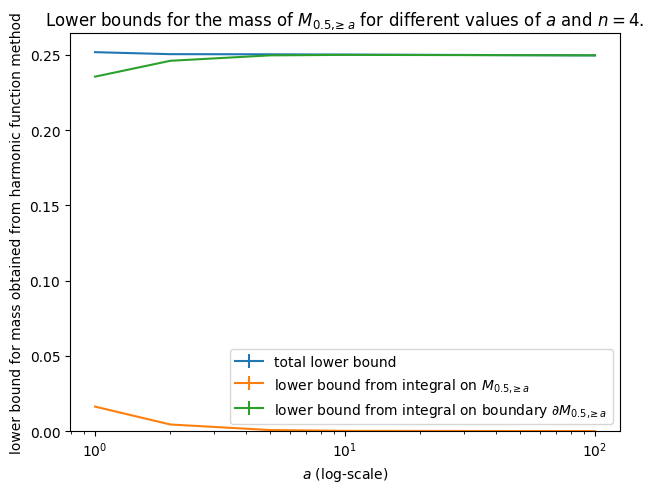
\includegraphics[width=0.8\linewidth]{figures/lower_bounds_for_different_values_of_a.png}
    \caption{}
    \label{fig:lower_bounds_for_different_values_of_a}
\end{figure}

And in fact by our argument in \cref{sec:condition_for_mass_equality} we should have equality between our lower bound and the mass, since \( u_3 \) has no critical points: We computed in our Jupyter Notebook, that
\begin{equation*}
    \partial_3 u_3=\frac{m x_{3}(a m + 2 x_{3} \abs{x}) -(m + 2 \abs{x}) (a m x_{3} - 2 \abs{x}^3)}{(m + 2 \abs{x})^{2} \cdot \abs{x}^2},
\end{equation*}
where the denominator is always positive (since \( a>0 \) and thus \( \abs{x}>0 \)) and where we we can express the numerator as
\begin{equation*}
    2x_3\cdot m\cdot \abs{x}\cdot (x_3-a)+(m+2\abs{x})\cdot 2\abs{x}^3,
\end{equation*}
which is also positive (since \( x_3\geq a \) and \( \abs{x}>0 \)). Thus \( \partial_3 u_3>0 \) everywhere on \( M_{m,\geq a} \) and there cannot be any critical points.

Thus \cref{sec:condition_for_mass_equality} yields that all level sets are (when intersected with our cylinders) diffeomorphic (as we can also obsere below in the plots of the level sets) and that the lower bound should be equal to the mass \( m/2=1/2 \) for all \( a>0 \).

\subsection{Plotting the harmonic level sets}
Using the same Jupyter notebook \parencite{fischerhenryrubenHarmonicFunctionMethod2023} as before, we also generate some plots of the level sets of \( u_2 \) (which look the same as those for \( u_1 \), just rotated) and of \( u_3 \) for \( M_{m,+} \) (see \cref{fig:level_sets_unmodified}) and of just \( x_3 \) for \( M_{m,\geq a} \) (but here for different \( a \)) (see \cref{fig:level_sets_modified})

Note that the method of plotting implicit surfaces we use here is susceptible to rounding errors and thus sometimes the level set if \( u_3 \) on \( M_{m,\geq a} \) corresponding to the boundary of the manifold is rendered with some slight imperfections (this specific level set should look flat in our coordinates). We can however symbolically verify even within the Jupyter notebook that in fact the boundary of the half-space is a level set.

Note also that even though in the level sets of the \( u_i=t \) for \( \abs{t}>0.5 \) on \( M_{m,+} \) there seem to be disconnected components of spherical / semi-spherical shape (seemingly contradicting our argument for \( \xi(S_t^L)\leq 1 \) directly preceding \cref{eq:starting_point_individual_computations}), this portion of the level set is entirely contained within the horizon boundary \( \Sigma \), \ie not contained in \( M(\Sigma) \), and thus surely also not in \( S_t^L\subset M(\Sigma) \).

Apart from helping in visualizing in particular how the boundary conditions (both asymptotic and on horizon and noncompact boundary) are fulfilled, these plots also show what we know from our discussion of the strength of the lower bounds above: 
\begin{itemize}
    \item For \( M_{m,\geq a} \) all the \( S_t^L \) (\ie the level sets when intersected with the filled half-cylinder \( \Omega_L \)) are diffeomorphic to a disk, and in particular \( \chi(S_t^L)=1 \). 
    \item \( M_{m,+} \) the \( S_t^L \) with \( t\in \interval{0}{m/2}=\interval{0}{0.5} \) have a different topology (they intersect the horizon boundary and are diffeomorphic to an annulus), while for \( t>m/2 \) all the \( S_t^L \) are diffeomorphic to a disk (as for \( M_{m,\geq a} \)). The change between these two happens at \( (0,0,m/2)=(0,0,0.5) \), where \( u_3 \) also has a critical point.
\end{itemize}

\begin{figure}
    \centering
    \begin{subfigure}{.49\textwidth}
        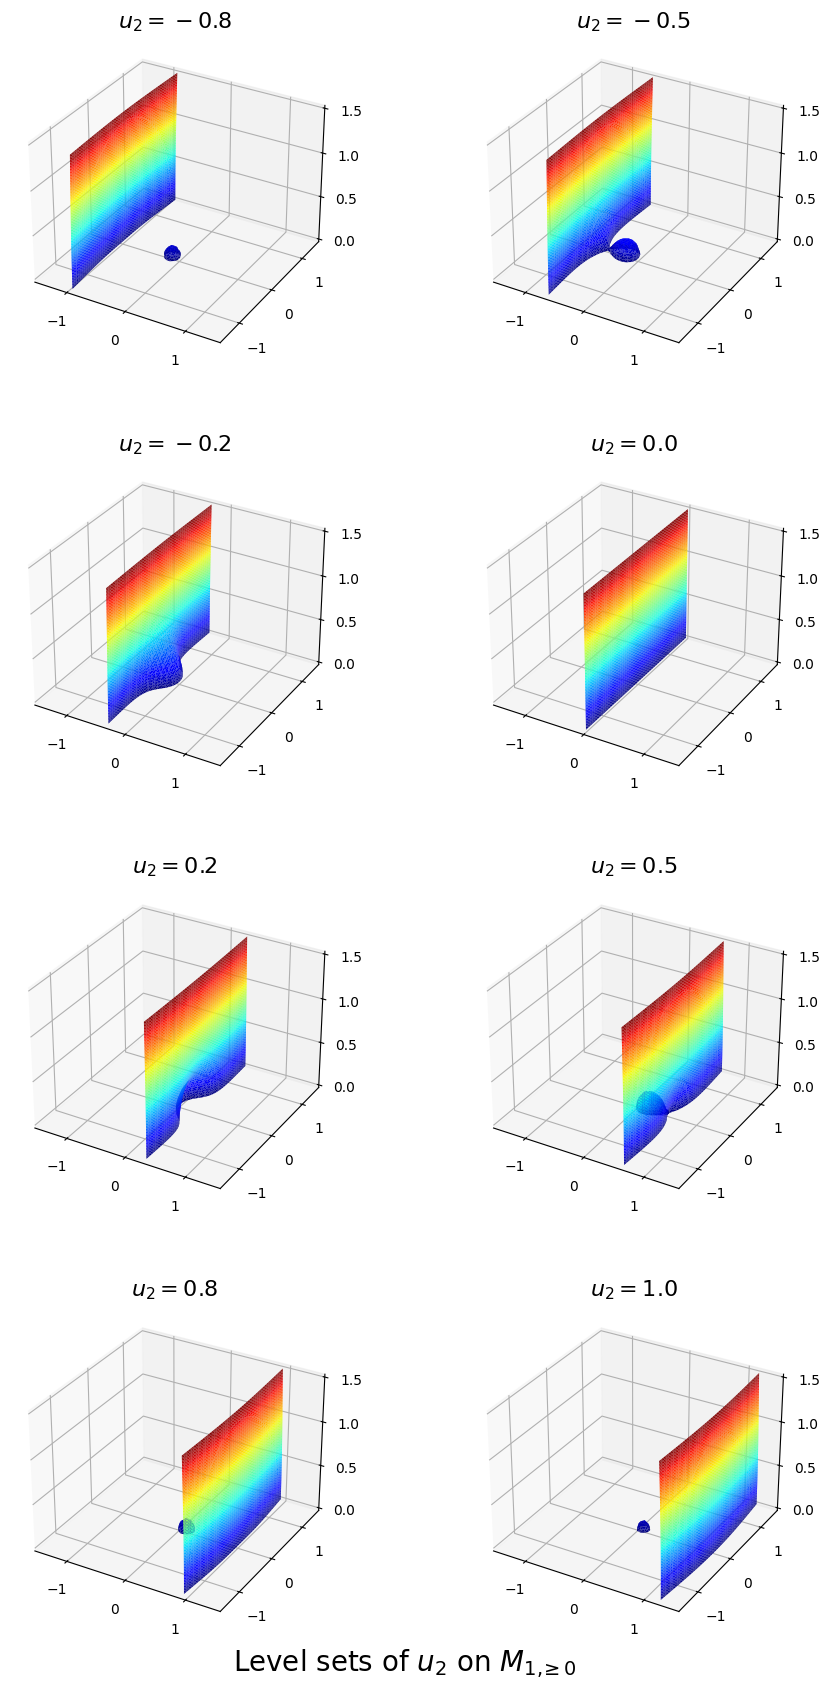
\includegraphics[width=\textwidth]{figures/level_sets_u2_unmodified.png}
    \end{subfigure}
    \begin{subfigure}{.49\textwidth}
        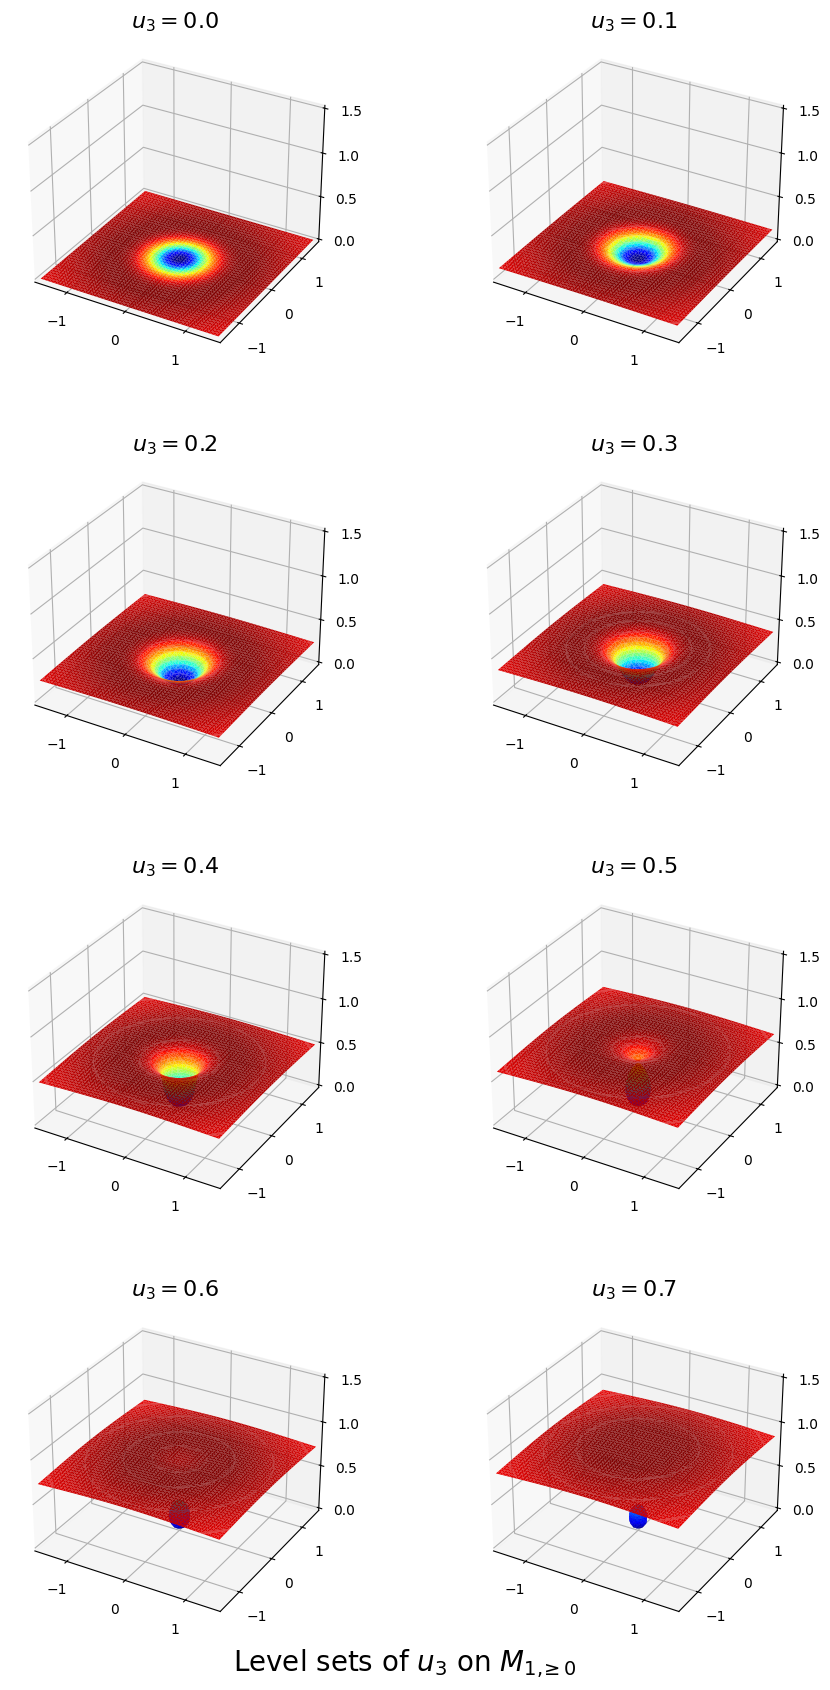
\includegraphics[width=\textwidth]{figures/level_sets_u3_unmodified.png}
    \end{subfigure}
    \label{fig:level_sets_unmodified}
    \caption{Level sets of harmonic coordinates \( u_i \) on \( M_{m,+} \). Note that for better visibility of any curvature, the height of points on the surfaces is also visualized using color.}
\end{figure}
\begin{figure}


    \centering
    \begin{subfigure}{.49\textwidth}
        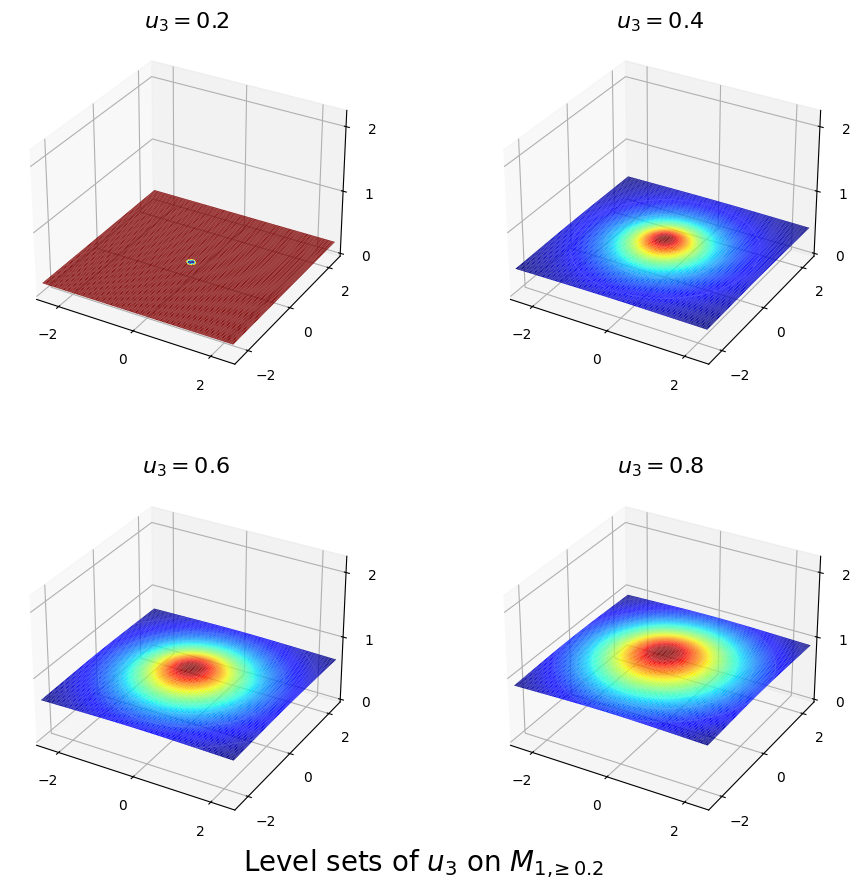
\includegraphics[width=\textwidth]{figures/level_sets_u3_modified_with_a_0.2.png}
    \end{subfigure}
    \begin{subfigure}{.49\textwidth}
        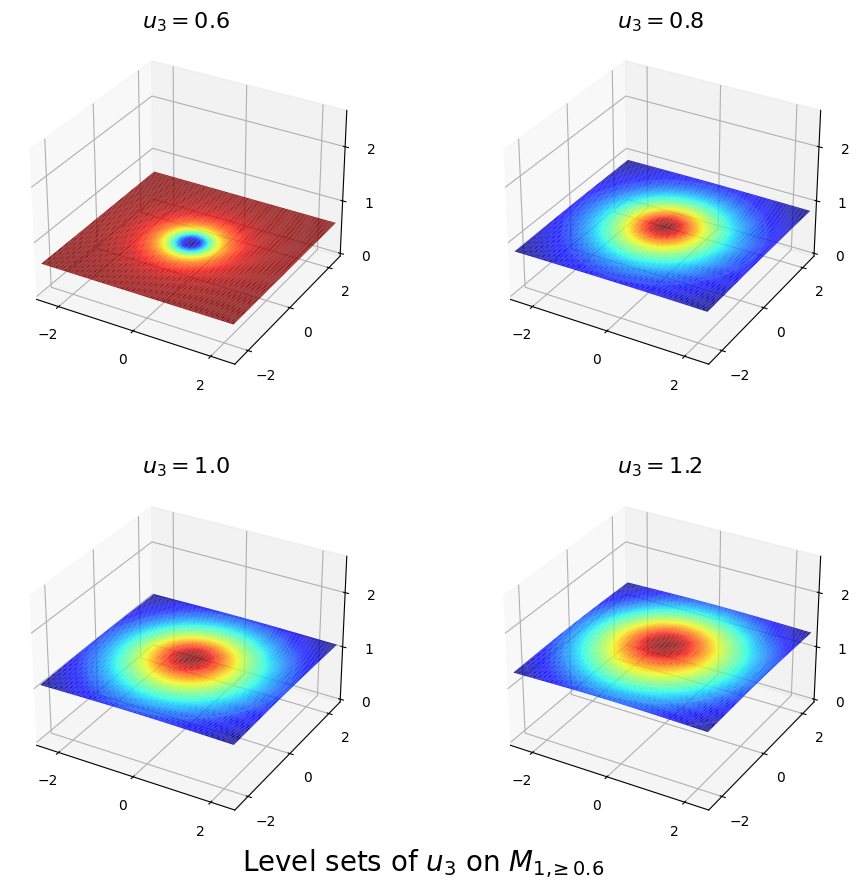
\includegraphics[width=\textwidth]{figures/level_sets_u3_modified_with_a_0.6.png}
    \end{subfigure}
    \begin{subfigure}{.49\textwidth}
        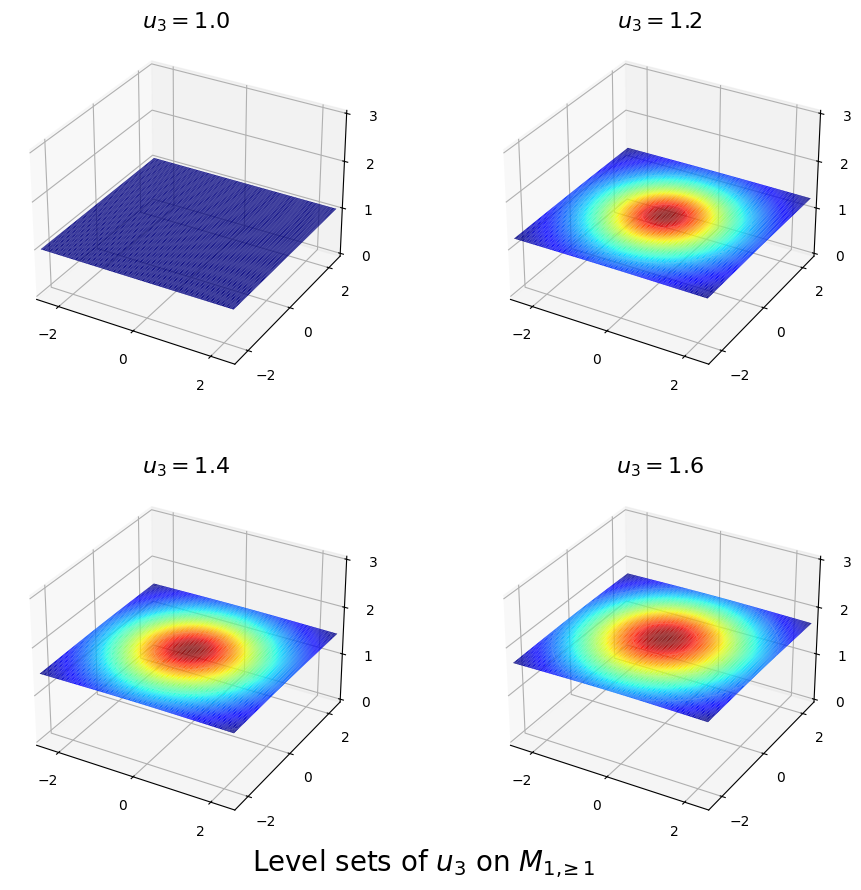
\includegraphics[width=\textwidth]{figures/level_sets_u3_modified_with_a_1.png}
    \end{subfigure}
    \label{fig:level_sets_modified}
    \caption{Level sets of \( u_3 \) on \( M_{m,\geq a} \) for different values of \( a \). Note that for better visibility of any curvature, the height of points on the surfaces is also visualized using color.}
\end{figure}
\todo{Decide whether I want acknowledgements.}
% \section{Acknowledgements}
% I want to thank in particular Prof.~Dr.~Thomas~Schick for supervising my thesis, suggesting the very interesting topic and for advising and helping me during the process. Thanks also to Professor Max Wardetzki for agreeing to be my second supervisor.
\newpage
\appendix
\section{Different Exhausting Sequences for Computation of the Mass}
\begin{proposition}\label{prop:mass_independent_of_exhausting_sequence}
    Suppose that \( (M,g) \) is an asymptotically flat half space with asymptotically flat coordinates \( x_1,x_2,x_3 \) on \( \Mend \) (fulfilling the conditions of \cref{def:half_space_mass}). Let \( \Set{D_k^3}_{k=1}^{\infty} \) be an exhaustion of \( M \) by closed sets with \( \boundary{D_k}=S_k\cup (D_k\cap \boundary{M}) \), where \( S_k \) is a connected \( 2 \)-dimensional piecewise smooth submanifold of the end \( \Mend \) with \( \boundary{S_k}=\boundary{M}\cap S_k \) such that
    \begin{gather*}
        R_k\definedas \inf_{x\in S_k} \abs{x}\goesto \infty\quad \text{as \( k\goesto \infty \)},\\
        R_k^2\cdot \abs{S_k} \text{ is bounded as \( k\goesto \infty \)},
    \end{gather*}
    and \( R_1\geq R_0 \), where \( \abs{S_k} \), the area of \( S_k \), and \( \abs{x} \) are as usual calculated with respect to the euclidean background metric (possible since we are in \( \Mend \)). Then
    \begin{equation*}
        \mass{M}{g}=\lim_{k \goesto \infty}\int_{S_k}\int_{\sphere_{r,+}^{2}}G_i\tilde{\mu}^i\odif{A}+\int_{\boundary{S_k}}g_{\alpha 3}\tilde{\theta}^\alpha\odif{l}
    \end{equation*}
    is independent of the sequence \( S_k \), where as in \cref{def:half_space_mass} \( \tilde{\mu}^i \) is the outward normal to \( S_k \) and \( \tilde{\theta}^\alpha \) the co-normal to \( \boundary{S_k} \) oriented as the boundary of the compact component of \( \boundary{M}\setminus \boundary{S_k} \).
\end{proposition}
\begin{proof}
    Let \( \tilde{D}_k\definedas \Set{x\in D_k\given \abs{x}\geq R_k} \) (this is the part of \( D_k \) extending beyond the biggest coordinate hemisphere that is possible to inscribe in \( D_k \)). Then \( \boundary{\tilde{D}_k}=S_k \cup \sphere^2_{R_k,+}\cup (\tilde{D}_k\cap \boundary{M}) \) and \( \boundary+{\tilde{D}_k\cap \boundary{M}}=(S_k\cap \boundary{M})\cup (\sphere^1_{R_k}) \).



    As in \cite[Proposition 3.7]{almarazPositiveMassTheorem2016}, we get (using \cite[Equations 3.16 and 3.17]{almarazPositiveMassTheorem2016})
    \begin{align*}
        \int_{\tilde{D}_k}{R}\odif{V}&=\begin{gathered}[t]
            \int_{S_k}G_i\tilde{\mu}^i \odif{A}-\int_{\sphere^2_{R_k,+}}G_i\mu^i\odif{A}\\
            +\int_{\tilde{D}_k \cap \boundary{M}}G_i\nu^i \odif{A}+\int_{\tilde{D}_k}\bigo{r^{-2\tau-2}},
        \end{gathered}\\
        \int_{\tilde{D}_k\cap \boundary{M}}G_i \nu^i\odif{A}&=\begin{gathered}[t]
            \int_{S_k\cap \boundary{M}}g_{\alpha 3}\tilde{\theta}^\alpha\odif{l}-\int_{\sphere{R_k}^1}g_{\alpha,3}\theta^\alpha\odif{l}\\
                -2\int_{\tilde{D}_k\cap \boundary{M}}H+\int_{\tilde{D}\cap \boundary{M}}\bigo{r^{-2\tau-1}},
        \end{gathered}
    \end{align*}
    and thus
    \begin{equation*}
        \begin{aligned}[t]
        &\rphantom{=}\abs[\Big]{\int_{S_k}G_i \tilde{\mu}^i \odif{A}+\int_{S_k\cap \boundary{M}}g_{\alpha 3}\tilde{\theta}^\alpha\odif{l}-\p[\Big]{\int_{\sphere^2_{R_k,+}}G_i\mu^i \odif{A}+\int_{\sphere^1_{R_k}}g_{\alpha 3}\theta^\alpha\odif{l}}}\\
        &\leq \int_{\tilde{D}_k}\bigo{r^{-2\tau-2}}+\abs{R}\odif{V}+\int_{\tilde{D}_k\cap \boundary{M}}\bigo{r^{-2\tau-1}}+\abs{H}\odif{A}\\
        &\leq \int_{M\setminus D_k}\bigo{r^{-2\tau-2}}+\abs{R}\odif{V}+\int_{(\boundary{M})\setminus D_k}\bigo{r^{-2\tau-1}}+\abs{H}\odif{A}\\
        \end{aligned}
    \end{equation*}
    Since \( R\in L^1(M) \) and \( H\in L^1(\boundary{M}) \), the fact that the \( D_k \) exhaust \( M \) (together with \( r>R_k \) in \( M\setminus D_k \)) implies that the integrals over \( R \) and \( H \) on the right hand side vanish in the limit \( k\goesto \infty \). Similarly, since \( \tau>1/2 \), the integrals over \( \bigo{r^{-2\tau-2}} \) and \( \bigo{r^{-2\tau-1}} \) also vanish in this limit. 
     
    We learn that using the \( S_k \) to compute the mass yields the same result as using coordinate spheres (as we used in our original \cref{def:half_space_mass}).
\end{proof}
\section{Basic Riemannian Geometry}\label{sec:basic_riemannian_geometry}
\begin{remark}\label{rem:manifolds_physicists_intuition}
    The following section will require some basic knowledge about manifolds, as \eg taught in \cite{leeIntroductionSmoothManifolds2012}. But in many physics courses a basic understanding / intuition for this topic is developed as well, via talking about different coordinate systems (called \emph{charts} in the language of differential geometry) and how objects transform between them. It should hopefully be possible to follow this introduction, and via that knowledge also the rest of this thesis, with only this \enquote{physicist's understanding of manifolds} and by ignoring any unfamiliar notation.

    The following are only some basic translation tools to understand the notation we will be using:
    \begin{itemize}
        \item A \( n \)-dimensional manifold \( M \) is some space which we can (at least locally) describe using \( n \) coordinates. Think \eg of the sphere with spherical coordinates \( (\varphi,\theta) \).
        \item \( \tangentspace{p}{M} \) is the collection of vectors tangent at \( p \) tangent to \( M \). 
        \item \( X\in \sheafsections{\tangentbundle{M}} \) is a \emph{vector field} on \( M \). In general a \( (k,l) \)-tensor (\( k \)-times covariant and \( l \)-times contravariant) \( T^{a_1\dotsm a_k}_{b_1\dotsm b_l} \) will be written as 
        \begin{equation*}
            T\in \sheafsections{\underbrace{\tangentbundle{M}\tensorproduct \tangentbundle{M}}_{l \text{-times}}\tensorproduct \underbrace{\cotangentbundle{M}\tensorproduct\dotsb\tensorproduct \cotangentbundle{M}}_{k \text{-times}}}.
        \end{equation*}
    \end{itemize}
\end{remark}
\begin{definition}\label{def:riemannian_metric}\label{def:riemannian_manifold}
    A \emph{Riemannian manifold} \( (M,g) \) is a smooth manifold \( M \) with a positive-definite, inner product \( g_p \) smoothly assigned to each point in \( M \), \ie a positive definite section \(g\in \sheafsections{\cotangentspace{M}\symmetricproduct \cotangentspace{M}} \) (where \( \symmetricproduct \) is the symmetric product). We call \( g \) a \emph{Riemannian metric}.
\end{definition}
\begin{remark}
    A \emph{Pseudo-Riemannian manifold} is equipped with a \emph{Pseudo-Riemannian metric} instead: Here the inner product on each tangentspace is not necessarily positive-definite anymore. We will most often consider \( 3+1 \)-dimensional \emph{Lorentzian manifolds}, where the metric has signature \( (-,+,+,+) \). We call the first coordinate the \emph{time coordinate} and the other three \emph{spacial coordinates}. All of the following constructions extend without modification to Lorentzian manifolds.
\end{remark}
\begin{remark}
    A metric allows us to convert between vectors and covectors, \ie we have an isomorphism (called the \emph{musical isomorphism})
    \begin{equation*}
        \tangentspace{p}{M}\to \cotangentspace{p}{M}\qquad v\mapsto v^\flat,
    \end{equation*}
    (with inverse \( \alpha\mapsto \alpha^{\sharp} \)), where for \( w\in \tangentspace{p}{M} \) we define
    \begin{equation*}
        v^{\flat}(w)=g(v,w).
    \end{equation*}
    In coordinates this map is given by lowering the index of our vector \ie \( v^a\rightsquigarrow g_{ab}v^b=v_a \).
\end{remark}
\begin{remark}
    Recall that on any manifold, we can always contract one covariant and one contravariant index of a tensor. This is equivalent to taking the trace of the endomorphism \( \tangentspace{p}{M}\to \tangentspace{p}{M} \) given by this \( \sheafsections{\tangentbundle{M}\tensorproduct \cotangentbundle{M}} \) part of the tensor.
    
    In the presence of a metric, the \emph{musical isomorphism} allows us to raise and lower arbitrary indices and thus contract (originally) covariant with covariant indices and contravariant with contravariant tensors, \ie if we have a tensor \( T_{ij\dotsc} \) we can compute the contraction \( \gtrace+{g}{T}_{\dotsc}=g^{ij}T_{ij\dotsc} \). This is equivalent to choosing an orthonormal basis \( X_i \) and dual basis \( X^i \) and evaluating
    \begin{equation*}
        \gtrace+{g}{T}(\cdots)=\sum_{i}T(X_i,X_i,\cdots).
    \end{equation*}
\end{remark}

Riemannian manifolds enable us to not only take derivatives of functions as is possible on all smooth manifolds, but of all tensor fields:
\begin{definition}
    A \emph{covariant derivative} (or sometimes \emph{(affine) connection}) is an \( \reals \)-linear map \( \nabla\maps \sheafsections{\tangentspace{M}}\to \sheafsections{\cotangentspace{M}\tensorproduct \tangentspace{M}} \) such that the product rule
    \begin{equation*}
        \nabla(f\cdot X)=\odif{f}\tensorproduct X+f\cdot \nabla X
    \end{equation*}
    is fulfilled for any function \( f \maps M\to \reals\). We often write \( \nabla_Y X \) for \( (\nabla X)(Y) \).

    The covariant derivative also extends to arbitrary tensors, such that for \( T \) a \( (k,l) \)-tensor, \( \nabla T \) is a \( (k,l+1) \) tensor. Here we demand 2 further properties:
    \begin{enumerate}
        \item \( \nabla(T\tensorproduct T')=\nabla T\tensorproduct T'+T\tensorproduct \nabla T' \), \ie a Leibniz rule for the tensor product.
        \item The covariant derivative commutes with taking traces (contracting a covariant and a contravariant part of a tensor):
        \begin{equation*}
            \nabla_Y (\trace{T})=\trace+{\nabla_Y(T)}.
        \end{equation*}
    \end{enumerate}
\end{definition}
\begin{notation}  \label{notation:derivative_indices}  
    We write \( T_{(\text{indices}),i} \) and \( T_{(\text{indices});i} \) for the partial and covariant derivative of \( T \) in the direction \( x_i \).
\end{notation}
\begin{remark}
    Note that \( \nabla_Y X \) is tensorial in \( Y \) (since \( \nabla X \) is a tensor), \ie if \( Y  \) is a vector field then \( (\nabla_Y X)(p) \) only depends on \( Y(p) \) at a point \( p\in M \). But \( \nabla_Y X \) is \emph{not} tensorial in \( X \), only linear (\ie \( \nabla_Y (X+aX')=\nabla_Y X+ a\nabla_Y X' \)), instead \( (\nabla_Y X)(p) \) depends on the behaviour of \( X \) around \( p \) (as is to be expected for a derivative)
\end{remark}
\begin{remark}
    If we set
    \begin{equation*}
        \nabla_Y f =\odif{f}(Y)=Y(f),
    \end{equation*}
    then the first product rule involving functions and vector fields is just another incarnation of our product rule for tensors.
\end{remark}
\begin{remark}
    We can define higher covariant derivatives, \eg
    \begin{equation*}
        \nabla^2_{X,Y}(Z)(\cdots)=(\nabla(\nabla Z))(X,Y).
    \end{equation*}
    In coordinates we can then compute that
    \begin{equation*}
        \begin{aligned}[t]
            (\nabla^2_{X,Y}Z)^a&=X^b Y^c \nabla_b\nabla_c Z^a\\
            &=X^b \nabla_b (Y^c \nabla_c Z^a)-(X^b \nabla_b Y^c)(\nabla_c Z^a)\\
            &=(\nabla_X \nabla_Y Z)^a-(\nabla_{\nabla_X Y}Z)^a.
        \end{aligned}
    \end{equation*}
    Note that, since coordinate vector fields commute, we have
    \begin{equation*}
        \nabla^2_{a,b}=\nabla_a \nabla_b-\nabla_b \nabla_a.
    \end{equation*}
\end{remark}

\begin{remark}
    Writing \( \nabla_i \) for \( \nabla_{\partial_i} \) in coordinates, we note that the covariant derivative differs from the (coordinate dependent) partial derivative by a linear correction term given by the \emph{Christoffel symbol} (also sometimes called the connection coefficients) \( \Gamma^a_{b c} \):
    \begin{equation*}
        \nabla_{a} X^b = \partial_a X^b+\Gamma_{ac}^b X^c.
    \end{equation*}
\end{remark}
\begin{recall}
    The commutator of two vector fields \( X,Y \) is another vector field fulfilling
    \begin{equation*}
        \commutator{X}{Y}(f)=X(Y(f))-Y(X(f)).
    \end{equation*}
\end{recall}
\begin{theorem}
    Let \( (M,g) \) be a Riemannian manifold. We call a connection \( \nabla \) the \emph{Levi-Civita connection} if it is
    \begin{enumerate}
        \item Metric compatible: \( \nabla g=0 \), and thus in particular
        \begin{equation*}
            \nabla_Z (g(X,Y))=g(\nabla_Z X, Y)+g(X,\nabla_Z Y),
        \end{equation*}
        \item Torsion free: For vector fields \( X \) and \( Y \) we have
        \begin{equation*}
            \nabla_Y X-\nabla_X Y=\commutator{X}{Y}.
        \end{equation*}
        This can also, in coordinates, be expressed as
        \begin{equation*}
            \Gamma^{a}_{bc} = \Gamma^a_{cb}.
        \end{equation*}
    \end{enumerate}
    There always exists a unique Levi-Civita connection on \( (M,g) \). Its coefficients in coordinates are (this is also called the Koszul formula)
    \begin{equation}
        \Gamma^a_{bc}=\frac{1}{2}g^{ad}(\partial_b g_{cd}+\partial_c g_{bd}-\partial_d g_{bc}).\label{eq:koszul_formula}
    \end{equation}
\end{theorem}

\begin{definition}
    We define the Laplacian (also called Laplace-Beltrami-Operator)
    \begin{equation*}
        \laplacian{f}=\gtrace+{g}{\nabla^2 f}=\nabla^a \nabla_a f.
    \end{equation*}
\end{definition}
\begin{lemma}\label{lem:laplacian_in_terms_of_metric_determinant}
    If \( M \) is Riemannian and equipped with the Levi-Civita-connection,
    \begin{equation*}
        \laplacian{f}=\frac{1}{\sqrt{\det{g}}}\partial_{a}(\sqrt{\det{g}}\partial^a f).
    \end{equation*}    
\end{lemma}
\begin{proof}
    Our proof proceeds entirely in coordinates. Note first that (for \( I \) the identity matrix)
    \begin{equation*}
        \det'(I)=\trace;.
    \end{equation*}
    Then consider the function
    \begin{equation*}
        f(A)=\det{A}=\det{g}\cdot \det(\inverse{g}\cdot A).
    \end{equation*}
    Taking the derivative and evaluating at \( A=g \) then gives
    \begin{equation*}
        \det'(g)(T)=\det{g}\cdot \trace{\inverse{g}\cdot T},
    \end{equation*}
    and thus
    \begin{equation*}
        \begin{aligned}[t]
            \partial_a \det{g}&=\det{g}\cdot \trace{\inverse{g}\cdot \partial_i g}\\
            &=\det{g}g^{bc}\partial_{a}g_{bc}.
        \end{aligned}
    \end{equation*}

    Thus we can compute
    \begin{equation*}
        \begin{aligned}[t]
            \Gamma^{a}_{ab}&=\frac{1}{2}g^{ac}(\partial_a g_{bc}+\partial_b g_{ac}-\partial_c g_{ab})\\
            &=\frac{1}{2}g^{bc}\partial_b g_{ac}\\
            &=\frac{1}{2\det{g}}\partial_b(\det{g})\\
            &=\frac{1}{\sqrt{\det{g}}}\partial_b(\sqrt{\det{g}}),
        \end{aligned}
    \end{equation*}
    where the second equality is due to the fact that (because of symmetry of \( g \))
    \begin{equation*}
        g^{ac}\partial_{a}g_{bc}=g^{ca}\partial_c g_{ba}.
    \end{equation*}

    Then    
    \begin{equation*}
        \begin{aligned}[t]
            \nabla^a \nabla_a f&= \partial_a \nabla^a f+\Gamma^a_{ab} \nabla^b f\\
            &=\frac{1}{\sqrt{\det{g}}}\cdot \sqrt{\det{g}}\partial_a(g^{ab} \partial_b f)+\frac{1}{\sqrt{\det{g}}}\cdot (\partial_b \sqrt{\det{g}})(g^{ab}\partial_b f)\\
            &=\frac{1}{\sqrt{\det{g}}}\partial_a(\sqrt{\det{g}}g^{ab}\partial_b f).
        \end{aligned}
    \end{equation*}
\end{proof}


One major difference between the covariant and our usual partial derivatives is that covariant derivatives in different directions do not necessarily commute. The failure of this commutativity is one way to understand and measure curvature:
\begin{definition}[Riemann curvature tensor]\label{def:riemann_curvature_tensor}
    We define the \emph{Riemann curvature tensor} 
    \begin{equation*}
        R\in \sheafsections{\cotangentbundle{M}\tensorproduct \tangentbundle{M}\tensorproduct \tangentbundle{M}\tensorproduct \tangentbundle{M}}
    \end{equation*} 
    by writing it as a map taking at each point three tangent vectors \( X,Y,Z \) and returning another tangent vector, which we denote by \( R(X,Y)Z \):
    \begin{equation*}
        \riemanncurvature(X,Y)Z\definedas \nabla^2_{X,Y}Z-\nabla^2_{Y,X}Z=\nabla_X \nabla_Y Z- \nabla_Y \nabla_X Z -\nabla_{\commutator{X}{Y}}Z.
    \end{equation*}
    The \( \nabla_{\commutator{X}{Y}}Z \) term ensures that \(  \riemanncurvature \) is a tensor. We denote \(  \riemanncurvature \) in coordinates by
    \begin{equation*}
        \riemanncurvature^d_{cab}Z^c=\nabla_a \nabla_b Z^d-\nabla_b \nabla_a Z^d.
    \end{equation*}
\end{definition}
\begin{remark}\label{rem:second_derivatives_function_commute}
    Note that we still have \( \nabla_a \nabla_b f=\nabla_b \nabla_a f \) for any function \( f \).
\end{remark}
Oftentimes, the \( 4 \) indices of the Riemann curvature tensor are both unwieldy to work with and not necessary to describe many phenomena. By contracting / taking traces we can get two further measures of curvature:
\begin{definition}
    We define the \emph{Ricci curvature} as
    \begin{equation*}
        \Ricci(X,Y)\definedas\trace+{X\mapsto R(X,Y)Z}
    \end{equation*}
    or, in coordinates,
    \begin{equation*}
        \Ricci_{ab}=\riemanncurvature^c_{acb}.
    \end{equation*}
\end{definition}
We will require the Ricci curvature only once during this thesis, as a stepping stone for our main integral inequality. A lot more important will be the scalar curvature, which in General Relativity is proportional to mass density for static spacetimes, and thus is central formulating the positive mass theorem in purely geometric terms:
\begin{definition}
    We define the \emph{scalar curvature} as
    \begin{equation*}
        R\definedas \gtrace{g}{\Ricci}=g^{ij}\Ricci_{ij}.
    \end{equation*}
\end{definition}

\section{Riemannian submanifolds}\label{sec:riemannian_submanifolds}

We will often be considering a three dimensional spacelike hypersurface (defined in \cref{def:spacelike_hypersurface})  \( M \) embedded in a larger \( 3+1 \)-dimensional Lorentzian manifold \( \tilde{M} \) (for the signature of the metric of \( \tilde{M} \) we choose the convention \( (-,+,+,+) \)), such that the induced metric on \( M \) is positive definite. \( M \) itself will also often have a boundary \( \boundary{M} \). Thus some basic facts about Riemannian submanifolds will be helpful. Most of the following is from \cite[Chapter~2.1]{leeGeometricRelativity2019}.

{ \newcommand{\Mconnection}{\nabla}\newcommand{\Sigmaconnection}{\hat{\nabla}}
Let \( \Sigma^m \) be a submanifold of (pseudo-)Riemannian manifolds \( (M^n,g) \) (equipped with Levi-Civita connection \( \Mconnection \)).
\begin{remark}
    \( g \) induces a metric
    \begin{equation}
        \gamma=\restrict{g}{\tangentbundle{\Sigma}}\label{eq:first_fundamental_form}
    \end{equation} 
    (also called the \emph{first fundamental form}) on \( \Sigma^m  \). 

    If \( \Sigma^m \) is Riemannian inside a Lorentzian manifold \( M^n \), \ie if the induced metric \( \gamma \) is positive definite, then we call \( \Sigma^m \) a \emph{spacelike submanifold}.\label{def:spacelike_hypersurface}
\end{remark}
This metric \( \gamma \) in turn defines a Levi-Civita connection on \( \Sigma \), which fulfills the following relation:
\begin{fact}
  Denoting the Levi-Civita connection of \( (\Sigma,\gamma) \) by \( \Sigmaconnection \), we have for any \( p\in \Sigma \), tangent vector \( X\in \tangentspace{p}{\Sigma} \) and \( Y\in \sheafsections{\tangentbundle{\Sigma}} \),
  \begin{equation*}
    \Sigmaconnection_X Y=(\Mconnection_X \tilde{Y})^\top,
  \end{equation*}
  where \( \tilde{Y} \) is any extension of \( Y \) to a vector field on \( M \). Here \( (\blank)^\top \) denotes the orthogonal projection from \( \tangentspace{p}{M} \) to \( \tangentspace{p}{\Sigma} \) (which in coordinates can be done via \( X^i\mapsto \gamma^i_j X^j \)).
\end{fact}
Thus \( \Sigma \) intrinsically contains information about tangential parts of tangential derivatives. But this information does not determine the orthogonal part! This motivates the following definition:
\begin{definition}[Second fundamental form]
    The \emph{second fundamental form} of \( \Sigma \) is a tensor \( \mathbf{A}\in \sheafsections{\cotangentbundle{\Sigma}\tensorproduct \cotangentbundle{\Sigma}\tensorproduct \normalbundle{\Sigma}} \) such that for \( X,Y\in \tangentspace{p}{\Sigma} \)
    \begin{equation*}
        \mathbf{A}(X,Y)\definedas (\Mconnection_X \tilde{Y})^\perp,
    \end{equation*}
    where \( (\blank)^\perp \) denotes the orthogonal projection from \( \tangentspace{p}{M} \) to the normal space \( \normalspace{p}{\Sigma} \). Here \( \tilde{Y} \) is again any extension of \( Y \) to a vector field on \( M \).
\end{definition}  
Note that although \( \Mconnection \) is not a tensor (\ie although it depends on the behaviour of the vector field \( \tilde{Y} \) around a point \( p \)), the second fundamental form \( \mathbf{A} \) \emph{is} tensorial. In both of the above definitions, we did not have to extend \( X \) to a vector field, since \( \Mconnection \) only depends on the value of \( X \) at \( p \).

\begin{fact}
    \( \mathbf{A}(X,Y)=\mathbf{A}(Y,X) \), \ie \( \mathbf{A} \) is symmetric, since for any extensions \( \tilde{X},\tilde{Y} \) of \( X,Y \) we have \( \Mconnection_X Y-\Mconnection_Y X=\commutator{X}{Y}\in \tangentspace{\Sigma} \).
\end{fact}
\begin{proof}
    Recall that when treating our vector fields as derivations we can also compute the Lie Bracket  as \( \commutator{X}{Y}(f)=X(Y(f))-Y(X(f)) \). This does obviously not depend on whether the ambient manifold of \( X \) and \( Y \) is \( \Sigma \) or \( M \), and thus the resulting vector field \( \commutator{X}{Y} \) must be a vector field on \( \Sigma \). 
\end{proof}
\begin{definition}
    The \emph{mean curvature vector} \( \mathbf{H} \) is the trace of \( \mathbf{A} \) over \( \tangentspace{p}{\Sigma} \), \ie for an orthonormal basis \( e_1,\dotsc,e_n \) of \( \tangentspace{p}{\Sigma} \) we define
    \begin{equation*}
        \mathbf{H}\definedas \sum_{i=1}^{m}\mathbf{A}(e_i,e_i).
    \end{equation*}
\end{definition}
\begin{definition}\label{def:geodesic_curvature}
    Let \( \Sigma\subset \Sigma'\subset M \) be a one-dimensional submanifold of a two-dimensional submanifold \( \Sigma' \) of some ambient manifold \( M \), let \( v \) be some normed tangent vector field of \( \Sigma \) and let \( n \) be a preferred choice of normal to \( \Sigma \) inside \( \Sigma' \) (oftentimes \( \Sigma \) will be the boundary of some region in \( \Sigma' \) and we will let \( n \) be the outward unit normal), then we define the \emph{(signed) geodesic curvature of \( \Sigma \) in \( \Sigma' \)} as
    \begin{equation}\label{eq:def_geodesic_curvature}
        \kappa_{\Sigma}=-\scalarproduct{\nabla_v v}{n}.
    \end{equation}
\end{definition}
\begin{definition}
    If \( \Sigma \) is an orientable hypersurface of \( M \), we can choose a normal direction \( \nu \) (if \( \Sigma \) has an interior and exterior, we typically implicitly choose \( \nu \) to be the outward normal). Then we define
    \begin{equation}
        A(X,Y)\definedas g(\mathbf{A}(X,Y),-\nu)\qquad H\definedas g(\mathbf{H},-\nu)=\gtrace{\gamma}+{A}.\label{eq:def_mean_curvature}
    \end{equation}
    We also call \( A \) the second fundamental form and \( H \) the mean curvature. 
\end{definition}
Note that we have
\begin{equation*}
    A(X,Y)=g(\nabla_X Y,-\nu)=\underbrace{\nabla_X (g(Y,-\nu))}_{=0}-g(Y,\nabla_X (-\nu))=g(Y,\nabla_X \nu).
\end{equation*}
Thus by using the projection \( \gamma^i_j \) we can write \( A \) in coordinates as
\begin{equation}
    A_{ij}=\gamma^k_i\gamma^l_j \nabla_k \nu_l.\label{eq:second_fundamental_form_in_coordinates}
\end{equation}
The above in particular also implies that
\begin{equation*}
    H=\divergence_g \nu,
\end{equation*}
if we extend \( \nu \) to a normal vector field in a neighborhood of \( \Sigma \). To see this, note that \( 0=\nabla_\nu(1)=\nabla_{\nu}(g(\nu,\nu)) \) implies \( g(\nu,\nabla_\nu \nu)=0 \).
\begin{remark}\label{rem:mean_curvature_peculiarities}
    With this definition, the mean curvature of a twodimensional surface is the sum of the principal curvatures, not the mean. Another common definition of the mean curvature is
    \begin{equation*}
        H=\frac{1}{n-1}\gtrace+{\gamma}{A},
    \end{equation*}
    where \( n \) is the dimension of the manifold \( M \), but most of our references use the same definition as we do.

    Note also that we follow in particular \cite{almarazPositiveMassTheorem2016} in choosing a sign convention for \( A \) and \( H \) opposite to that of their classical definition (given some normal \( \nu \)). See also \cite[Remark 2.1]{leeGeometricRelativity2019} for why this choice is usually made.
\end{remark}
We are now equipped to express an important formula relating the curvature of \( \Sigma \) to the curvature of \( M \). 
\begin{lemma}
    Let \( \riemanncurvature,\tilde{\riemanncurvature} \) denote the Riemann curvature of \( M \) and \( \Sigma \) respectively.
    For \( X,Y,Z,W \in \tangentspace{\Sigma}\), the \emph{Gauss-Codazzi equation} states
    \begin{equation}
        \scalarproduct{\riemanncurvature_(X,Y)Z}{W}=\scalarproduct{\tilde{\riemanncurvature}(X,Y)Z}{W}+A(X,Z)A(Y,W)-A(X,W)A(Y,Z)\label{eq:gauss_codazzi}
    \end{equation}
    or in coordinates
    \begin{equation}
        \gamma^{i}_{i'}\gamma^j_{j'}\gamma^k_{k'}\gamma^l_{l'}\riemanncurvature_{ijkl}=\tilde{\riemanncurvature}_{i'j'k'l'}+A_{i'k'}A_{j'l'}-A_{i'l'}A_{j'k'}\label{eq:gauss_codazzi_coordinates}.
    \end{equation}
    Contracting with \( g^{i'k'}\gamma^{j'l'} \) also yields
    \begin{equation}
        \Ricci(\nu,\nu)=\frac{1}{2}(R_M-R_{\Sigma}+H^2-\abs{A}^2). \label{eq:contracted_gauss_codazzi}
    \end{equation}
\end{lemma}

The following (which is \cite[Exercise 2.3 in][]{leeGeometricRelativity2019}) is the main fact we will require to deal with calculations on the non-compact boundary of our objects of interest (asymptotically flat half-spaces):
\begin{fact}\label{fact:laplacian_and_hypersurface_laplacian}
    Given a hypersurface \( \Sigma \) in \( (M,g) \) and a smooth function \( f \) on \( M \),
    \begin{equation*}
        \laplacian_M f=\laplacian_\Sigma +\Mconnection_\nu\Mconnection_\nu f+H \Mconnection_\nu f.
    \end{equation*}
\end{fact}
\begin{proof}
    Choose an orthonormal frame \( e_1,\dotsc,e_n \) of \( \tangentspace{p}{M} \) and \( e_1,\dotsc,e_{n-1}\in \tangentspace{p}{\Sigma} \) and \( e_n=\nu \), then
    \begin{align*}
        \laplacian_M f&=\sum_{i=1}^{n}(\Mconnection\Mconnection f)(e_i,e_i)\\
        &=\Mconnection_M \Mconnection_\nu f+\sum_{i=1}^{n-1}g(\Mconnection_{e_i} (\grad_M f),e_i)\\
        &=\Mconnection_\nu \Mconnection_\nu f+\sum_{i=1}^{n-1}g(\Mconnection_{e_i}(\grad_{\Sigma}f+\nu\cdot \Mconnection_\nu f),e_i)\\
        &=\begin{aligned}[t]
            &\Mconnection_\nu \Mconnection_\nu f+\sum_{i=1}^{n-1}(\gamma(\Sigmaconnection_{e_i}(\grad_{\Sigma} f),e_i)+\underbrace{g(\mathbf{A}(e_i,\grad{\Sigma}),e_i)}_{=0}\\
            &+\Mconnection_{
        e_i}\Mconnection_{\nu}f\cdot \underbrace{g(\nu,e_i)}_{=0}+\Mconnection_{\nu}f\cdot g(\Mconnection_{e_i}\nu,e_i))
        \end{aligned}\\
        &=\Mconnection_\nu \Mconnection_\nu f+\sum_{i=1}^{n-1}(\Sigmaconnection\Sigmaconnection f)(e_i,e_i)+\Mconnection_\nu f\cdot \sum_{i=1}^{n-1}A(e_i,e_i)\\
        &=\Mconnection_\nu \Mconnection_\nu f+\laplacian_{\Sigma}f+\Mconnection_{\nu}f\cdot H.
    \end{align*}
\end{proof}
}
\section{Miscellaneous definitions and results}\label{sec:miscellaneous}

\subsection{Gauss-Bonnet and the Euler characteristic}
One of the main reasons for why the current technique does not readily seem to extend to higher dimensions is its reliance on applying the following theorem (which is specific to two dimensions) to level sets of harmonic functions on three-dimensional space:
\begin{theorem}[Gauss-Bonnet Theorem]\label{thm:gauss_bonnet}
    Let \( \Sigma \) be a compact two-dimensional Riemannian manifold with boundary \( \boundary{\Sigma} \). Let \( R \) be the scalar curvature of \( \Sigma \) and let \( \kappa_{\boundary{\Sigma}} \) be the geodesic curvature of \( \boundary{\Sigma} \) in \( \Sigma \). Then
   \begin{equation*}
    \int_\Sigma R/2 \odif{A}+\int_{\boundary{\Sigma}}\kappa_{\boundary{\Sigma}}\odif{t}=2\pi \chi(\Sigma),
   \end{equation*} 
   where \( \chi(\Sigma) \) is the Euler characteristic (for a definition see below) of \( \Sigma \).
\end{theorem}
For a proof see \cite[Chapter 4.3]{petersenRiemannianGeometry2006}. 

\begin{definition}[Euler Characteristic]
    For a compact, connected, oriented surface \( \Sigma \) (two-dimensional manifold with boundary), the \emph{Euler characteristic} is given by
    \begin{equation}
        \chi(\Sigma)=2-2g-b,\label{eq:def_euler_characteristic}
    \end{equation}
    where \( g\geq 0 \) is the genus and \( b \) is the number of connected boundary components.

    For non connected surfaces \( \Sigma=\bigsqcup_{i\in I} \Sigma_i \), where the \( \Sigma_i \) are the connected components of \( \Sigma \), we have
    \begin{equation*}
        \chi(\Sigma)=\sum_{i}\chi(\Sigma_i).
    \end{equation*}

    If a non-compact space \( S \) results from a puncture of a compact space (is homotopy equivalent to \( \sigma\setminus \Set{x_1,\dotsc,x_p} \), where \( p \) is the number of punctures), then we set
    \begin{equation}
        \chi(S)=\chi(\Sigma)-p.\label{eq:def_euler_characteristic_non-compact}
    \end{equation}
\end{definition}
The following theorem (a version of the maximum principle) will then help control the Euler characteristic of the level sets of our harmonic functions:
\begin{theorem}\label{thm:maximum_principle}
 Let \( \Omega \) be a compact connected Riemannian manifold with boundary \( \boundary{\Omega}=P_1\sqcup P_2 \). Let \( u\maps \Omega\to \reals \) be harmonic (\ie \( \laplacian u=0 \)) with Dirichlet boundary condition \( u= 0 \) on \( P_1 \) and Neumann boundary condition \( \partial_n u=0 \) on \( P_2 \), where \( n \) is normal to \( P_2 \).

 Then \( u=0 \) on all of \( \Omega \).
\end{theorem}
\begin{proof}
    We start from
    \begin{equation*}
        0=\int_\Omega u\cdot \laplacian u\odif{\Omega}.
    \end{equation*}
    Integrating by parts then yields
    \begin{align*}
        0&=\int_\Omega u\cdot g^{ij}\nabla_i \nabla_j u\odif{x}\\
        &=\int_\Omega \nabla_i u\cdot g^{ij} \nabla_j u\odif{x}-\int_{\boundary{\Omega}}u\cdot g^{ij}\nabla_i u \cdot n_j \odif{S}\\
        &=\int_\Omega \abs{\nabla u}^2\odif{x}-\int_{\boundary{\Omega}}u\cdot \partial_n u\odif{S}.
    \end{align*}
    But we always have either \( u=0 \) or \( \partial_n u=0 \) on \( \boundary{\Omega} \), and we conclude that \( \abs{\nabla u}=0 \) everywhere, \ie that \( u \) is constant on \( \Omega \) (since \( \Omega \) only has one connected component).
\end{proof}

\subsection{Bochner's identity}
A major ingredient that allows us to connect the derivatives of our harmonic functions to the curvature of the surrounding space is Bochner's identity:
\begin{lemma}\label{lem:bochner_identity}
    For any smooth function \( u \) on a Riemannian manifold \( (m,g) \),
    \begin{equation*}
        \frac{1}{2}\laplacian(\abs{\nabla u}^2)=\abs{\nabla^2 u}^2+g(\grad (\laplacian u),\grad u)+\Ricci(\grad u, \grad u).
    \end{equation*} 
\end{lemma}
\begin{proof}
    A straightforward calculation in coordinates yields
    \begin{equation*}
        \begin{aligned}[t]
            \frac{1}{2}\laplacian \abs{\nabla u}^2&=\frac{1}{2}\nabla^j\nabla_j(\nabla_i u \nabla^i u)\\
            &=\nabla^j((\nabla_j \nabla_i u)(\nabla^i u))\\
            &=(\nabla^j \nabla_j\nabla_i u)(\nabla^i u)+(\nabla_j \nabla_i u)(\nabla^j \nabla^i u)\\
            &\explain{\text{\cref{rem:second_derivatives_function_commute}}}{=}\nabla^j((\nabla_i \nabla_j u)(\nabla^i u))\\
            &=(\nabla_j \nabla_i \nabla^j u)(\nabla^i u)+\abs{\nabla^2 u}^2\\
            &\explain{\text{see \cref{def:riemann_curvature_tensor}}}{=}(\nabla_i \nabla_j \nabla^j u+\riemanncurvature_{kji}^j \nabla^k u)(\nabla^i u)+\abs{\nabla^2 u}^2\\
            &=g(\grad \laplacian u,\grad u)+\abs{\nabla^2 u}^2+\Ricci_{kj}(\nabla^k u)(\nabla^j u)\\
            &=\abs{\nabla^2 u}^2+g(\grad (\laplacian u),\grad u)+\Ricci(\grad u, \grad u).
        \end{aligned}
    \end{equation*}
\end{proof}
\subsection{The mean curvature under conformal changes of metric}\label{sec:conformal_changes_of_metric}
In \cref{sec:example} we consider the Schwarzschild half-space as an example. In that context we also have to compute the mean curvature of some surfaces. But, since the Schwarzschild metric is conformal to the euclidean metric, we are able to simplify our calculations in \cref{sec:example} using a formula derived below. For a more in depth treatment of conformal transformations, see \cite{curryIntroductionConformalGeometry2015}.


In the following, let \( (M,\bar{g}) \) always be conformal to \( (M,g) \), \ie let \( \bar{g}=\Omega^2 g \) for some real function \( \Omega \). Denote all quantities with a bar (\eg \( \bar{\nabla},\bar{R},\bar{H} \)) when they are computed with respect to \( \bar{g} \) and without a bar when they are computed with respect to \( g \). Let \( \Sigma \) be some hypersurface of \( M \) with normal vectors \( \nu,\bar{\nu} \). Second fundamental forms \( A,\bar{A} \) and mean curvatures \( H,\bar{H} \) will follow the definitions from \cref{eq:def_mean_curvature}.

\begin{lemma}\label{lem:conformal_change_connection}
    \begin{equation*}
        \bar{\nabla}_X Y =\nabla_X Y+X(f)\cdot Y+Y(f)\cdot X-g(X,Y)\grad{f}.
    \end{equation*}
\end{lemma}
\begin{proof}
    We will be using the Koszul formula \cref{eq:koszul_formula},
    \begin{equation*}
        \Gamma^a_{bc}=\frac{1}{2}g^{ad}(\partial_b g_{cd}+\partial_c g_{bd}-\partial_d g_{bc}).
    \end{equation*}
    In particular we note that (since \( \bar{g}^{ad}=e^{-2f}g^{ad} \))
    \begin{equation*}
        \bar{\Gamma}^c_{ab}\begin{aligned}[t]
            &=\frac{1}{2}e^{-2f}g^{cd}(\partial_a(e^{2f}g_{bd})+\partial_b(e^{2f}g_{ad})-\partial_d(e^{2f}g_{ab}))\\
            &=\Gamma^c_{ab}+\delta^c_a\partial_b f +\delta^c_b\partial_a f-g_{ab}\nabla^c f.
        \end{aligned}
    \end{equation*}
    Then
    \begin{equation*}
        \begin{aligned}[t]
            (\bar{\nabla}_X Y)^c&=X^a \bar{\nabla}_a Y^c\\
            &=X^a \partial_a Y^c + X^a\bar{\Gamma}_{ab}^c  Y^b\\
            &=X^a \partial_a Y^c +X^a \Gamma_{ab}^c Y^b+X^c Y^b \partial_b f+ Y^c X^a \partial_a f-\nabla^c f g_{ab}X^a Y^b\\
            &=(\nabla_X Y)^c+X^c\cdot Y(f)+Y^c\cdot X(f)-\nabla^c f \cdot g(X,Y),
        \end{aligned}
    \end{equation*}
    as required.
\end{proof}
\begin{lemma}\label{lem:mean_curvature_under_conformal_transform}
    \begin{equation*}
        \bar{H}=e^{-f}(H+(n-1) g(\grad f,\nu)).
    \end{equation*}
\end{lemma}
\begin{proof}
    Let \( e_1,\dotsc,e_n \) be an orthonormal basis at some tangent space under \( g \) such that \( e_1,\dotsc,e_{n-1}\in \tangentspace{\Sigma} \), then \( \bar{e}_a=e^{-f}e_a \) is such an orthonormal basis under \( \bar{g} \). Similarly we have \( \bar{\nu}=e^{-f}\nu \). 

    We can then compute     
    \begin{equation*}
        \bar{A}(X,Y)\begin{aligned}[t]
            &=\bar{A}(X,Y)\\
            &=\bar{g}(\bar{\nabla}_X Y,-e^{-f}\nu)\\
            &=e^{f}[A(X,Y)+X(f) g(Y,-\nu)+Y(f) g(X,-\nu)-g(\nabla f,-\nu)\cdot g(X,Y)]
        \end{aligned}
    \end{equation*}
    This then leads directly to
    \begin{equation*}
        \bar{H}\begin{aligned}[t]
            &=\sum_{\alpha=1}^{n-1}\bar{A}(\bar{e}_\alpha,\bar{e_\alpha})\\
            &=\sum_{\alpha=1}^{n-1}e^{-2f}\bar{A}(e_\alpha,e_\alpha)\\
            &\explain[big]{g(e_{\alpha},\nu)=0}{=}\sum_{\alpha=1}^{n-1}e^{-f}(A(e_i,e_i)+0+0-g(\grad f,-\nu)\cdot 1)\\
            &=e^{-f}(H+(n-1)\cdot g(\grad f,\nu)).
        \end{aligned}
    \end{equation*}
\end{proof}
% \section{Python code for computations and graphs}
% \lstinputlisting[language=Python,frame=lines,caption={Numerical computation of the mass lower bound for the Schwarzschild examples},label={lst:computations_and_graph_for_example},basicstyle=\footnotesize]{computations_and_graphs/computations_and_graphs.py}
\printbibliography
\newpage
\thispagestyle{empty}
\vspace*{1cm}
\vfill  % Selbstständigkeitserklärung
~\\
\begin{large} % Schriftgroße = large (sonst normal)
\textbf{Selbstständigkeitserklärung}
\end{large}
~\\
Hiermit erkläre ich, dass ich die vorliegende Arbeit
selbstständig und nur unter Verwendung der angegebenen
Quellen und Hilfsmittel verfasst habe.\\
~\\
Göttingen, den 30.09.2023 \hspace*{4cm} \begin{tabular}{l}
    {}\\
    \makebox[2.5in]{\hrulefill}\\
    Henry Ruben Fischer \end{tabular}
\end{document}